\documentclass[12pt,a4paper]{article}
\usepackage[utf8]{inputenc}
\usepackage{amsmath}
\usepackage{amsfonts}
\usepackage{amssymb}
\usepackage{graphicx}
\graphicspath{ {images/} }
\usepackage{algorithm}
\usepackage[noend]{algpseudocode}
\usepackage{hyperref}
\usepackage[table,xcdraw]{xcolor}
\usepackage{subcaption}
\usepackage{colortbl}
\usepackage{hhline}
\hypersetup{
    colorlinks,
    citecolor=black,
    filecolor=black,
    linkcolor=blue,
    urlcolor=black
}


\newcommand\tab[1][1cm]{\hspace*{#1}}

\makeatletter
\def\BState{\State\hskip-\ALG@thistlm}
\makeatother

% Default fixed font does not support bold face
\DeclareFixedFont{\ttb}{T1}{txtt}{bx}{n}{12} % for bold
\DeclareFixedFont{\ttm}{T1}{txtt}{m}{n}{12}  % for normal

% Custom colors
\usepackage{color}
\definecolor{deepblue}{rgb}{0,0,0.5}
\definecolor{deepred}{rgb}{0.6,0,0}
\definecolor{deepgreen}{rgb}{0,0.5,0}

\usepackage{listings}

% Python style for highlighting
\newcommand\pythonstyle{\lstset{
language=Python,
basicstyle=\tiny ,
morekeywords={self},              % Add keywords here
keywordstyle=\tiny\color{deepblue},
emph={MyClass,__init__},          % Custom highlighting
emphstyle=\tiny\color{deepred},    % Custom highlighting style
stringstyle=\color{deepgreen},
frame=tb,                         % Any extra options here
showstringspaces=false
}}


% Python environment
\lstnewenvironment{python}[1][]
{
\pythonstyle
\lstset{#1}
}
{}

% Python for external files
\newcommand\pythonexternal[2][]{{
\pythonstyle
\lstinputlisting[#1]{#2}}}

% Python for inline
\newcommand\pythoninline[1]{{\pythonstyle\lstinline!#1!}}
\renewcommand{\contentsname}{Indice}

\begin{document}
\begin{titlepage}
	\centering
	{
\includegraphics[scale=0.5]{logo}\par}
	\vspace{1cm}
	{\bfseries\large ESCUELA TÉCNICA SUPERIOR DE INGENIERÍA INFORMÁTICA \par}
	\vspace{1cm}
	{\scshape\large DOBLE GRADO INGENIERIA DEL SOFTWARE + MATEMÁTICAS\par}
	\vspace{1cm}
	{\bfseries\large Curso Académico 2021/2022 \par}
	\vspace{1cm}
	{\bfseries\large  Trabajo Fin de Grado \par}
	\vspace{2cm}
	{\scshape\large ESTUDIO DE DIVERSIFICACIÓN DE INVERSIONES SOBRE IBEX-35 UTILIZANDO CLUSTERING\par}
	\vspace{2cm}
	\vfill
	{\normalsize\textbf Autor: \par}
	{\normalsize Javier Méndez García-Brioles \par}
	{\normalsize\textbf Directores: \par}
	{\normalsize Regino Criado \par}
\end{titlepage}





	\vspace{1cm}
	\tableofcontents

\pagebreak
	
	\vspace{1cm}
	\section{Resumen}
	\vspace{1cm}
Este proyecto tiene como finalidad proponer un plan de inversión alternativo para minimizar la volatilidad de la inversión, y por tanto, minimizar el riesgo.\\
El plan de inversión consiste en aplicar una modificación del algoritmo k-means para agrupar los stocks en k clusters y de esos clusters sacar un optimo, dando lugar a k stocks diferentes en los que invertir.\\
Con esté plan haremos un estudio sobre los stoks del IBEX-35 comparando nuestro algoritmo con planes de inversión convencionales para ver como se consigue la mínima volatilidad. Ademas haremos un estudio de previsión para ver si nuestro algoritmo mantiene la mínima volatilidad si añadimos datos posteriores a los que tiene como input el algoritmo.\\
Además facilitaremos una interfaz gráfica para mostrar e interactuar con los datos.\\
\pagebreak
	\vspace{1cm}
	\section{Objetivos}
	\vspace{1cm}
Desde siempre ha existido la necesidad de comparar datos y ver su relación entre ellos, y una muy buena forma de ejercer esta comparación es clasificando los estos datos en conjuntos de datos. Dentro de cada conjunto los datos tienen mayor relación entre ellos que con los datos de fuera del conjunto, pero la búsqueda de estos conjuntos no es fácil. En la actualidad a esta búsqueda se la denota como clustering, que es puede considerar como el proceso por el cual se crean conjuntos de elementos similares. Este proceso se puede aplicar sobre todo conjunto de datos sobre los que se pueda aplicar una comparación entre ellos pero en este caso nos centraremos en buscar clusters de ondas temporales mediante varios métodos que comentaremos a continuación.\\
En un principio nos íbamos a basar en el grafo de visibilidad sacado de cada stock para, mediante sus propiedades, agrupar estos stocks. Pero al decidirnos por agrupar los stocks mediante k-means, la transformación a grafo de visibilidad ha pasado a un segundo plano, sirviendo como medio para transformar nuestras series iniciales a otras series que recojan las propiedades de los grafos de visibilidad.\\
Partimos de un conjunto de elementos, los cuales están compuestos por una sucesión de valores a lo largo de un intervalo de tiempo, estos elementos se pueden clasificar tal cual, o se puede hacer una transformación antes de su clasificación y utilizar esa transformación como input. En nuestro caso exploraremos 3 caminos:\\
1 Realizamos la clasificación sobre los elementos sin transformar.\\
2 Transformamos los elementos en una versión simplificada de ellos mismos para intentar mejorar el tiempo de ejecución.\\
3 Transformamos los elementos en su correspondiente grafo de Visibilidad y luego aplicamos el algoritmo sobre esos grafos.\\
Este proyecto se basara en la clasificación de series temporales mediante una variación sobre un método muy conocido llamado K-Means, lo que nos permite clasificar elementos siempre que se pude definir una función distancia entre ellos.\\
Una vez que tenemos nuestros elementos separados en distintos conjuntos, después de hacer las transformaciones y aplicar el algoritmo K-means tenemos k conjuntos cuyos elementos son similares entre ellos, esto resulta muy útil ya que nuestros elementos de entrada son stocks, por lo tanto saber que stocks se parecen entre ellos nos permite evitar elegir stocks que se comportan de forma parecida lo que nos permite minimizar la volatilidad de la inversión.
Por último, una vez llegado al resultado que es la volatilidad de la inversión podremos comparar todos los caminos que hemos utilizado entre ellos y con resultados de control (como son invertir de forma homogénea en todos los stocks, invertir todo en el stock menos volátil o invertir en n stocks aleatorios) para ver así que variación del método es el mejor o si los resultados de control son superiores.\\
Durante todo el proyecto trabajaremos sobre los datos producidos por las empresas dentro del IBEX-35 y proporcionados por una API de yahoo finances.\\
Desde un punto de vista más teórico nos centraremos en evolucionar el algoritmo K-means para que se adecue a nuestras necesidades, lo que consiste en hacer modificaciones para que el K-means acepte distancias un poco menos convencionales que la genérica, ejecutar el K-means varias veces para mejorar la precisión de los conjuntos y por ultimo modificar K-means para que también funcione sobre un grafo.\\


	\vspace{1cm}











	\vspace{1cm}
	\section{Fundamentos Teóricos}
	\vspace{1cm}
		\subsection{Ondas Temporales}
			{\textbf{Ondas Simples}}\\
			Llamaremos ondas simples a las cuales compuestas exclusivamente por una función seno, con sus posibles modificaciones de amplitud, frecuencia, y desplazamiento.\\
			{\textbf{Ondas Compuestas}}\\
			Llamaremos ondas compuestas a la superposición de ondas simples a lo largo del tiempo\\
			{\textbf{Transformada de Fourier}}\\
			La transformada de Fourier es una función matemática que permite relacionar un dominio temporal con un dominio de frecuencias en ambos sentidos\\
			{\textbf{Transformada Wavelet}}\\
			La transformada Wavelet es una función muy utilizada en compresión de imágenes que permite dividir la cantidad de valores manteniendo la mayor cantidad posible de detalle.\\
		\subsection{Teoría de Grafos}
			{\textbf{Grafo}}\\
			Un grafo  ($G = (V,E)$) es una estructura de datos compuesta por vértices ($V$), donde se almacenan los datos, y aristas o arcos ($E=V\times V$), que representan las conexiones entre dos vértices.\\
			{\textbf{Grafo no Dirigido}}\\
			Grafo  ($G = (V,E)$) tal que:
			\[ V \neq \emptyset \]
			\[ E\subseteq \{ (a,b) / (a,b)\in E \rightarrow (b,a)\in E  \}  \]
			{\textbf{Vértice}}\\
			Componente mínimo indivisible por el que están compuestos los grafos\\
			{\textbf{Arista}}\\
			Componente de un grafo que se caracteriza por conectar dos vértices (E)\\
			{\textbf{Grado}}\\
			El grado de un vértice ($v\in V$) es:
			\[degre(v)=|E_v|\]
			\[ E_v\subseteq \{ (a,b)\in E / a=v \lor b=v \}  \]
			{\textbf{Orden}}\\
			El orden de un grafo ($G = (V,E)$) es:
			\[orden(G)= degre(w)\]
			con\\
			\[ w\in V / \forall v\in V      degre(w) \geq  degre(v)  \]
			{\textbf{Grafo de Visibilidad}}\\
			Un grafo de visibilidad es el grafo asociado a una onda temporal siguiendo el siguiente proceso:\\
			-A cada valor de la onda se le asigna un nodo del grafo.\\
			-Las conexiones se deciden según que nodos se ven entre ellos sin que otro nodo les bloque la visión. Esta restricción equivale a cumplir la ecuación ($y_m + \frac{y_n-y_m}{n-m}(k-m) \geq y_k$) para todo nodo k entre m y n ($ m < k < n$)\cite{GrafoVisibilidad} \\

		\subsection{Centralidad}
			La centralidad en un grafo consiste en la asignación de un número a cada nodo del grafo, este valor es sumamente importante ya que permite comparar nodos entre sí.\\
			La importancia de la centralidad reside en que encontrando nodos con valores muy altos de centralidad es equivalente a encontrar los nodos más importantes del grafo, los cambios a estos nodos causarán el mayor impacto dentro del grafo. Este valor es externo al propio nodo y puede variar con cualquier modificación del grafo, aunque esa modificación no afecte al grafo en sí.\\
			La centralidad es de suma importancia pues nos permite estudiar las conexiones entre objetos, ya sea entre personas a través de medios como las redes sociales, o las conexiones por carretera entre ciudades. Y este estudio por ejemplo nos permite saber la influencia de cierta persona x, o el trafico probable en una ciudad.\\
			Hay varias medidas que se pueden usar para determinar la centralidad, pero nosotros nos vamos a centrar en la centralidad de grado y la interpolación(Betweenness)\\
			{\textbf{Centralidad de grado}}\\
				La centralidad de grafo es posiblemente la medida de centralidad más fácil de entender. Consiste en contar el número de conexiones que tiene cada nodo, lo cual nos basta para ver si un nodo esta incomunicado o cual es la distancia entre cualquier pareja de nodos del grafo. Estos son datos muy útiles para el estudio de grafos, pero para ciertas aplicaciones se nos quedan cortos.\\ 
			{\textbf{Intermediación}}\\
				La intermediación es un poco más compleja y consiste en calcular el numero de veces que un nodo se utiliza como puente en la ruta más corta entre una pareja de nodos. Pongamos el ejemplo de una red de ordenadores, el nodo con una intermediación más alta seria por el cual pasa más información, sabiendo esto podemos ver que si ese nodo se incapacita sería el que más problemas ocasionaría a la red. Por lo tanto, con esta información podríamos saber los nodos que necesitan más protección en todo momento, esto es algo que con un simple estudio del grado de cada nodo no se vería.\\

		\subsection{Distancias}

		Una distancia es cualquier función que cumple lo siguiente:\\
			\begin{enumerate}
			\item $d(x,y) = 0 \iff x = y $
			\item $d(x,y) =d(y,x)$ (simetría)
			\item $d(x,z) \leq d(x,y) + d(y,z)$ (desigualdad triangular)
			\end{enumerate}
			Lo que nos dice de forma análoga por la desigualdad triangular:\\
			$d(x,y)\geq 0$ (no negatividad)\\

		\subsection{Volatilidad}
		La volatilidad es un termino que mide la variación de los valores a lo largo del tiempo, a mayor variación mayor volatilidad. Nuestra definición especifica de volatilidad va a ser bastante estándar.\\
		Definimos volatilidad como:\\
		\[Volatilidad = \sum_{i=1}^{n} \sqrt{\left | valor_i - media \right |} \]

		\subsection{Complejidad Computacional }
		Toda la teoría de Complejidad Computacional consiste en hacernos la pregunta, ¿que tareas son fáciles y que tareas son difíciles para un ordenador?. Al hacernos esta pregunta nos damos cuenta de no hay forma fácil de responder con lógica convencional ya que una tarea fácil para un ser humano no equivale a una tarea fácil para un ordenador. Pongamos como ejemplo reconocimiento de imágenes, si tenemos una imagen de un perro y se la enseñamos a una persona sabrá al momento que es un perro aunque no haya visto nunca esa foto exacta. \\
Pero para un ordenador eso resultaría imposible sin un gran trabajo por detrás y aunque en la actualidad ya existen algoritmos que permitan responder esa pregunta no están ni de lejos a la altura de una persona. \\
A su vez si tenemos cualquier tarea de computación pura un ordenador tardará mucho menos que  una persona. Así que resumiendo hay tareas fáciles para personas que nos casi imposibles para ordenadores y tareas fáciles para ordenadores que son casi imposibles para personas. \\
Por lo tanto para llegar a alguna conclusión vamos a necesitar una estrategia precisa que nos facilite algún indicador de que tareas son fáciles para un ordenador y eso es lo que hace el estudio de la Complejidad Computacional.\\
		 El estudio de la Complejidad se basa principalmente en estudiar dos parámetros, la cantidad de memoria utilizada por un algoritmo, y el numero de instrucciones que se ejecutan, esto equivale a medir el espacio y tiempo que gasta un algoritmo. Nosotros solo nos vamos a centrar en el estudio del tiempo.\\
		 
		Para un algoritmo concreto podemos definir la siguiente función T(n) a la cual le pasamos un input de tamaño n y nos devuelve el número de operaciones que realiza el algoritmo en el peor de los casos.\\
		\[T: N \rightarrow R^+ \]
		Como un ordenador realiza estas operaciones muy rápido los errores de magnitud pequeña pueden ser ignorados haciendo que solo nos importe el comportamiento asintótico de la ecuación conforme n crezca. Para expresar esto utilizaremos las siguientes definiciones.\\
		Sean $T, S : N \rightarrow R^+$ se dice que T(n) \textbf{domina} a S(n) si existen $k > 0$ y $n_o$ tal que para todo $n>n_0$:\\
		\[S(n) \leq kT(n) \]
		Con O(T(n)) siendo el conjunto de funciones dominadas por T(n) podemos decir que dos funciones T(n) y S(n) son \textbf{del mismo orden} si $ S(n) \in O(T(n)) y T(n) \in O(S(n))$.\
		Se llama \textbf{complejidad de un algoritmo} al mayor orden O(n) al que pertenece T(n).\\ 
		Dependiendo de cual sea el mayor O(n) al que pertenece T(n) podemos hablar de distintas complejidades. 
			\begin{enumerate}
			\item Con $T(n) \in O(log(n))$ se dice que el algoritmo tiene \textbf{complejidad logarítmica}
			\item Con $T(n) \in O(n)$ se dice que el algoritmo tiene \textbf{complejidad lineal}
			\item Con $T(n) \in O(n^2)$ se dice que el algoritmo tiene \textbf{complejidad cuadrática}
			\item Con $T(n) \in O(n^x)$ se dice que el algoritmo tiene \textbf{complejidad polinomial}
			\item Con $T(n) \in O(e^n)$ se dice que el algoritmo tiene \textbf{complejidad exponencial}
			\end{enumerate}
		

		\subsection{Algoritmos}
		{\textbf{Algoritmo de Dijkstra}}\\
		También conocido como algoritmo de mínimos caminos nos permite determinar el camino más corto entre un nodo origen y el resto de los nodos del grafo, si se hace este algoritmo sobre todos los nodos nos queda como resultado la mínima distancia entre todos los pares de nodos. Aquí se muestra su pseudocódigo:\\
			    \begin{algorithm}[H]
			    \caption{Algoritmo de Dijkstra}\label{euclid}
			    \hspace*{\algorithmicindent} \textbf{Input: {\normalfont   Grafo} ${G = (V,E)} $}\\
			    \textbf{\tab \tab {\normalfont \quad Nodo inicial}  ${node\_init}$}\\
			    \hspace*{\algorithmicindent} \textbf{Output:{\normalfont \quad Distancias} $\mathcal{D}=\{d_1..d_n\}$} 
			    \begin{algorithmic}[1]
			    \Procedure{Dijkstra}{${G},node\_init$}
			    \BState $\mathcal{D}=\{ d_1..d_n \} \gets \{INF..INF\}$
			    \BState ${pred} \gets \{\emptyset..\emptyset\}$
			    \BState ${seen} \gets \{False..False\}$
			    \BState ${D[node\_init]} \gets 0$
			    \BState \# \textit{Utilizamos una cola para asegurar el recorrido total del grafo}
			    \BState Q.add(node\_init,D[node\_init])
			    \BState \textbf{while}  ${Q \neq \emptyset }  \textbf{ do}$:
			    \State \# \textit{Extraer elemento de mínima distancia}
			    \State $node \gets Q.min()$
			    \State $seen[node] \gets True$

		            \For{$v \in adjacent(node)$} \do
			    \State \State 	\# \textit{Añadimos distancia si es menor que la actual}
				    \If {(\textbf{not} seen[v] \textbf{and} $\mathcal D[v] > \mathcal D[node] + E[node,v]$ )}
					\State $\mathcal D[v] \gets \mathcal D[node] + E[node,v]$
					\State $pred[v] \gets node$
			    		\State Q.add(v,D[v])
				    \EndIf
		            \EndFor
			    \BState \textbf{return} D;
			
			    \EndProcedure
			    \end{algorithmic}
			    \end{algorithm}
		Este algoritmo tiene una complejidad computacional $\mathbf{O(n^2)}$ ya que para cada nodo se puede llegar a recorrer todos los nodos. Pero si queremos saber las distancias entre todos los nodos la complejidad computacional aumenta a  $\mathbf{O(n^3)}$ pues hay que ejecutar el algoritmo de Dijkstra para cada nodo.\\
		{\textbf{K-means}}\\
		El K-means o K-medias es un método de clasificación no supervisada que permite la clasificación de n elementos en k grupos distintos, en cada uno de estos k grupos los elementos dentro se consideran más parecidos entre ellos que con los elementos de fuera. K-means se centra en resolver un problema de optimización en el cual se busca minimizar la suma total de la distancia de los elementos a su centroide más cercano:
		\[\min_{C} \sum_{i=1}^{k}\sum_{x_{j}\in C_{i}} d(\sigma_i , x_{j})\]
		Donde $d(x,y)$ es la función distancia utilizada,  $\{x_1..x_n\}$ son los elementos, $C=\{C_1..C_k\}$ son los k clusters y $\{\alpha_1..\alpha_k\}$  son los centroides correspondientes a cada cluster.\\
			La principal ventaja del k-means es que es muy rápido, pero tiene también una gran desventaja que hay que tener en cuenta, los resultados obtenidos dependen enormemente de como se inicializan los centroides. Por esta razón no podemos asegurar un optimo global sino que nos tendremos que conformar con un optimo local.\\
			K-means consta de 3 partes indispensables:\\
			\begin{enumerate}
			\item \textbf{Inicialización de centroides}: Se determinan las posiciones iniciales de los centroides, esto se puede hacer de muchas formas, todas ellas validas y todas ellas pueden dar soluciones ligeramente distintas. Podemos elegir por ejemplo los k primeros elementos como centroides o elegirlos de forma aleatoria.\\
			\item \textbf{Relacionar cada elemento con un centroide}: Para cada elemento se calcula la distancia a todos  los centroides y se relaciona con el centroide más cercano. Cada elemento se añade al cluster del centroide correspondiente.\\
			\item \textbf{Actualizar centroides}: Se actualizan los centroides haciendo la media de todos los elementos de su cluster y ese valor es el nuevo centroide.\\
			\end{enumerate}
			Los pasos 2 y 3 se repiten hasta que llegamos a nuestra condición de parada, que suele ser que la diferencia entre los centroides anteriores y los nuevos centroides sea menor a un valor umbral.\\
			
			El proceso se puede ver con más detalle en el siguiente pseudocódigo:\\
\pagebreak
			    \begin{algorithm}
			    \caption{K-means clustering}\label{euclid}
			    \hspace*{\algorithmicindent} \textbf{Input: {\normalfont   Data} $\mathcal{X} = \{x_1..x_n\}$}\\
			    \textbf{\tab \tab {\normalfont \quad Numero de clusters}  ${k}$}\\
			    \textbf{\tab \tab {\normalfont \quad Valor umbral}  ${ \varepsilon }$}\\
			    \hspace*{\algorithmicindent} \textbf{Output:{\normalfont \quad Clusters} $\mathcal{C}=\{C_1..C_k\}$} 
			    \begin{algorithmic}[1]
			    \Procedure{K-means}{$\mathcal{X},k,\varepsilon$}
			    \BState $\mathcal{C}=\{C_1..C_k\} \gets \{\emptyset..\emptyset\}$
			    \BState $ \{\sigma_1..\sigma_k\}  \gets$ \textbf {InicializarCentroides}($\mathcal{X},k$)
			    \BState \textbf{loop}:
			    \State \# \textit{Distribución de elementos en clusters}
			    \State $C_i \gets \{x_j / d(\sigma_i,x_j)  \leq d(\sigma_h,x_j) \forall h  \in \{1..k\}  \}  \forall i  \in \{1..k\}$
			    \State \# \textit{Actualización de clusters}
			    \State $new\sigma_i \gets \frac{\sum_{x_j\in C_i}x_j}{|C_i|} \forall i  \in \{1..k\}$
			    \State \# \textit{Comprobar la condición de parada}
			    \If {($ \sum_{i=1}^{k} d(\sigma_i,new\sigma_i) \leq  \varepsilon$)}
			    \State \Return $\mathcal{C}$
			    \EndIf
			    \State $ \{\sigma_1..\sigma_k\}  \gets \{new\sigma_1..new\sigma_k\}$
			    \State \textbf{goto} \emph{loop}.
			    \BState \textbf{close};
			    \EndProcedure
			    \end{algorithmic}
			    \end{algorithm}
			Para este algoritmo es difícil estudiar su complejidad computacional ya que el camino para llegar a la condición de parada es difícil de definir, por eso mismo se le considera un problema computacionalmente difícil (NP-hard), se han demostrado cotas de su complejidad como $\mathbf{O(n^{34}k^{34}d^8 log^4(n)/\sigma^6) }$ o $\mathbf{O(dn^4M^2)}$ para casos más simples, pero nosotros nos referiremos a su complejidad como $\mathbf{O_{K-means}}$ para poder compárala con la complejidad de las modificaciones al algoritmo\\
\pagebreak
	\vspace{1cm}






	\vspace{1cm}
	\section{Herramientas}
	\vspace{1cm}
Para este proyecto crearemos una aplicación python mediante la cual interactuaremos con la funcionalidad implementada, para esta implementación utilizaremos las siguientes herramientas:\\
\subsection{Anaconda}
Anaconda es una plataforma que gestiona entornos python para facilitar la instalación y uso de librerías python. Anaconda se centra en facilitar la programación científica, lo que incluye ciencia de datos, aprendizaje maquina y procesado de datos. Esto lo consigue implementando otra forma de instalar librerías a través del comando conda que equivale a el pip normal de python pero se centra en prevenir conflictos en la instalación de librerías, lo que produce un entorno más resistente a fallos de compatibilidad de librerías que con python convencional.\\
\subsection{Spyder}
Spyder es el IDE (Entorno de desarrollo integrado) que utilizaremos para la mayor parte de la programación. Viene por defecto con una gran cantidad de librerías integradas que resultan muy útiles para el desarrollo de código científico, como puede ser numpy o pandas. Ademas como es un entorno de código abierto, es decir, que permite que cualquiera pueda cambiar y distribuir el código, lo que hace que tenga una gran variedad de extensiones muy útiles para el desarrollo software.\\
\subsection{Extensiones Integradas en Spyder}
Aquí mencionaremos las principales extensiones que se han utilizado en el desarrollo de este proyecto:\\
-Spyder-Unittest: Es una extensión sobre Spyder que permite la automatización de test unitarios sobre nuestro código, ademas esta funcionalidad viene con una interfaz propia que permite la ejecución de todos los tests implementados a la vez y así poder ver al momento cuales fallan y cuales pasan.\\
-Spyder-GitHub: Es una extensión que permite acceder a GitHub desde dentro del entorno de desarrollo Spyder, lo que proporciona una pequeña interfaz gráfica para hacer commits y ver el historial del repositorio, ademas de permitir el uso de los comandos git dentro del terminal de Spyder.\\
-Spyder-Code Análisis: Esta extensión no da información sobre la calidad del código, muestra tanto las diferencias con las convenciones de como programar en python como las warnings y las vulnerabilidades del código.\\
-Spyder-Profiler: Esta extensión simplemente permite ver como está distribuido el tiempo de ejecución de la aplicación. El tiempo de ejecución se separa por método, lo que permite ver que métodos están consumiendo más recursos y esto ayuda en el proceso de optimización del código.\\
\subsection{Qt Designer}
Qt Designer es una herramienta que facilita el diseño de aplicaciones python aportando entorno donde poder crear, ver y gestionar la interfaz de una aplicación python. Este interfaz que se crea aquí se pude convertir en código python, el cual a su vez puede ser modificado en cualquier entorno de desarrollo python para añadir funcionalidad real a la aplicación. Qt Designer permite el uso de la librería gráfica QT en python lo que nos da opciones útiles que no nos dan otras librerías de interfaces de python como puede ser tkinter.\\
\subsection{Trello}
Trello es una aplicación con acceso web que permite la administración de proyectos. Se basa en un modelo kanban para poder llevar un seguimiento de las tareas a realizar en el desarrollo de nuestra aplicación.\\
\subsection{Github}
Github es un sistema de control de versiones que permite tener el código subido a un repositorio mientras que los cambios se hacen en local. Esto si se hace bien ayuda mucho en el desarrollo del código porque nos permite compartimentar cada parte de la funcionalidad en un commit individual que explique lo que se ha implementado en el mismo. Esto permite tener un buen historial de desarrollo para mejorar la mantenibilidad del código y permite tener versiones de código anteriores en caso de que durante el desarrollo rompamos la versión que tenemos del código en local y no sepamos arreglarlo, en este caso siempre podemos volver a la versión anterior del código para solucionar el problema.\\
\subsection{Programa Para Diagramas UML}
Este programa nos permite la creación de diagramas UML (lenguaje unificado de modelado) para poder mostrar una gran cantidad de relaciones distintas, por ejemplo la relación de las clases de nuestro programa, los casos de uso desde el punto de vista de un usuario o el diagrama de flujo que sigue el programa.\\
\subsection{LaTex}
Sistema de composición de textos que permite  la creación de documentos en formato estructurado y con eso se facilita el uso de elementos matemáticos y pseudocódigo en la memoria.\\
\pagebreak


		\section{Proceso}
		\subsection{Input}
			\subsubsection{Formato}
		Antes siquiera de pensar en hacer nada tenemos que dejar claro como son nuestros datos de entrada que vamos a estudiar.\\
		Lo primero de todo es tener claro que nuestro input son series temporales, es decir, una sucesión de valores ordenados a lo largo de un intervalo de tiempo como podemos ver a continuación:\\
\begin{figure}[H]
\centering
\begin{minipage}{.5\textwidth}
  \centering
  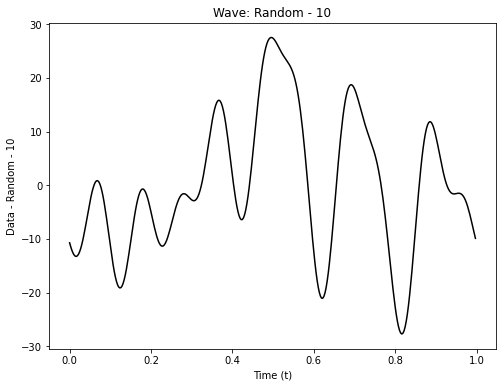
\includegraphics[width=.9\linewidth]{artificial serie}
  \caption{Serie artificial generada \\superponiendo 10 ondas simples\\ \phantom{filler}}
  \label{fig:test1}
\end{minipage}%
\begin{minipage}{.5\textwidth}
  \centering
  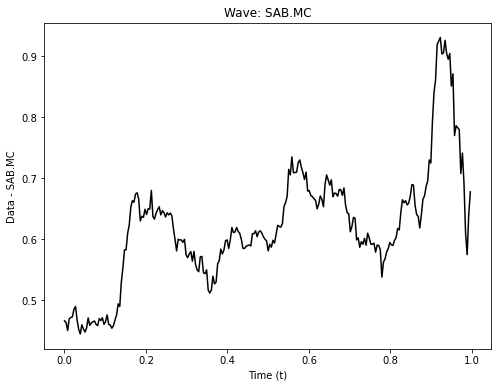
\includegraphics[width=.9\linewidth]{real serie}
  \caption{Serie real sacada de los valores de bolsa del banco Sabadel a lo largo del 2021}
  \label{fig:test2}
\end{minipage}
\end{figure}
		Estos valores en nuestro caso concreto equivalen al Valor de Apertura de un stock en un día concreto. Recogemos este valor diario durante un intervalo de tiempo, por defecto 1 año, y con eso tenemos una serie temporal vinculada a cada stock.\\
		Lo primero que hacemos con este conjunto de series temporales que tenemos como entrada es normalizarlas para facilitar su comparación. Esto consiste en:\\
		Considerando la serie S como la función
		\[\begin{array}{lcc}
		S:\mathbb{N}\rightarrow\mathbb{R}\\
 		\ \ \ \ \ t\rightarrow S(t)
		\end{array}\]
		La serie normalizada se corresponde a
		\[\begin{array}{lcc}
		S_n:\mathbb{N}\rightarrow(0,1]\\
 		\ \ \ \ \ \ \ t\rightarrow \frac{S(t)}{max(S)}
		\end{array}\]
		Lo que conseguimos con esto es que todas las series sean de magnitud comparable sin comprometer el comportamiento de la serie, ya que las subidas y bajadas de los valores se mantienen proporcionales a los valores antes de la normalización como podemos ver a continuación:\\
\begin{figure}[H]
\centering
\begin{minipage}{.5\textwidth}
  \centering
  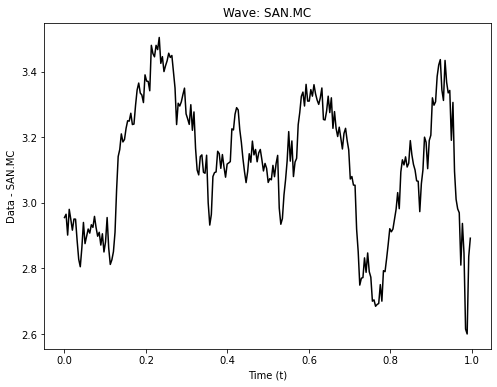
\includegraphics[width=.9\linewidth]{serie}
  \caption{Serie sacada de los valores\\ de bolsa del banco Santander a lo\\ largo del 2021}
  \label{fig:test1}
\end{minipage}%
\begin{minipage}{.5\textwidth}
  \centering
  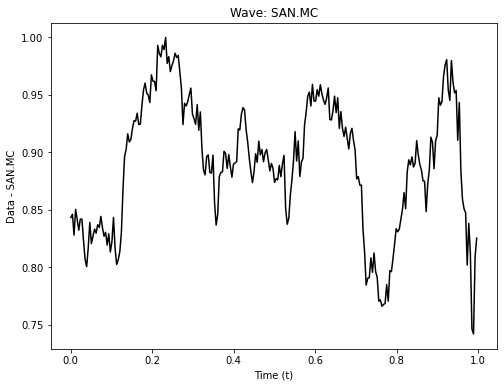
\includegraphics[width=.9\linewidth]{serie normalizada}
  \caption{Misma serie Normalizada\\ \phantom{filler}\\ \phantom{filler}}
  \label{fig:test2}
\end{minipage}
\end{figure}
		Como podemos ver la gráfica es idéntica, tan solo cambia la escala.\\
		Una vez que tenemos las series normalizadas ya están en posición de ser comparadas aplicando nuestro algoritmo que explicaremos más adelante, pero antes podemos aplicar otras transformaciones para mejorar el tiempo de ejecución, o para ver si hacen que nuestras series se comporten de forma distinta ante el algoritmo.
			\subsubsection{Fourier}
			La transformada de Fourier consiste en trasladar una función en dominio de tiempo, como son nuestras series temporales, a una función en dominio de frecuencia. En nuestro caso como trabajamos con valores finitos utilizamos la transformada de Fourier Discreta que da resultados aproximados a los que daría la transformada para funciones continuas. \\
			
\begin{figure}[H]
\centering
\begin{subfigure}{.5\textwidth}
  \centering
  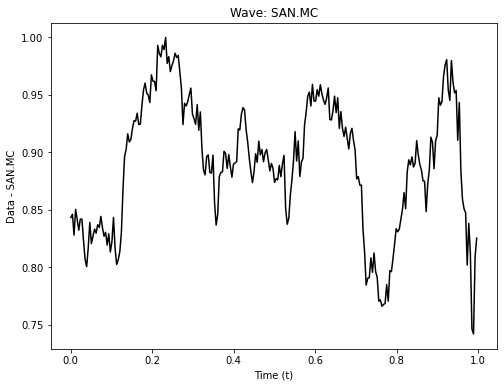
\includegraphics[width=.9\linewidth]{serie normalizada}
  \label{fig:sub1}
\end{subfigure}%
\begin{subfigure}{.5\textwidth}
  \centering
  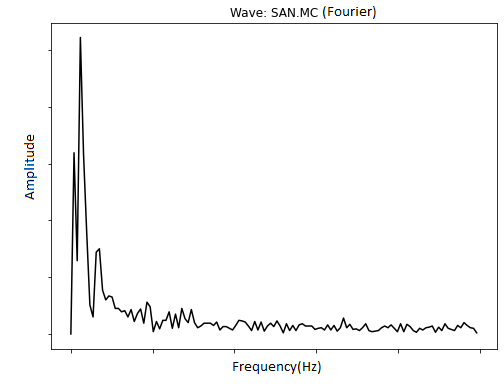
\includegraphics[width=.9\linewidth]{serie fourier}
  \label{fig:sub2}
\end{subfigure}
\caption{Transformada de Fourier}
\label{fig:test}
\end{figure}

			Esta transformación nos puede ser muy útil ya que nos puede reducir la cantidad de puntos a analizar, así que es una opción para mejorar el tiempo de ejecución de nuestro algoritmo. Pero tenemos que tener asegurarnos que los resultados al aplicar fourier son similares a los resultados sin aplicarlo, lo tendremos que estudiar más adelante.
			
			\subsubsection{Wavelet}
			En nuestro caso como hemos dicho antes trabajamos con un número finito de valores por lo tanto en este caso también necesitamos utilizar una versión discreta de la transformada Wavelet.\\
			La transformada Wavelet discreta  se utiliza mucho para la codificación y compresión de señales, por lo que es una buena opción para reducir el tamaño de nuestro input.\\
			El proceso se basa en dividir la serie temporal en dos nuevas series con la mitad de valores cada uno, una serie recoge las trazas principales de la serie temporal y la otra los detalles más pequeños como podemos ver a continuación:\\
\begin{figure}[H]
\centering
\begin{subfigure}{.5\textwidth}
  \centering
  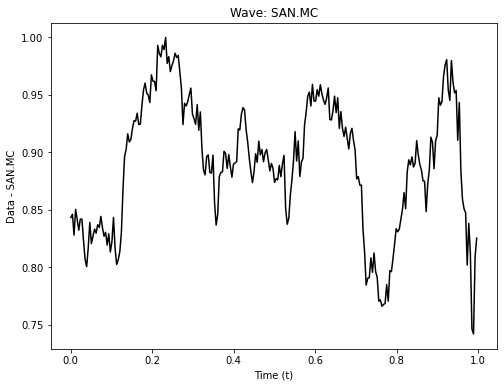
\includegraphics[width=.9\linewidth]{serie normalizada}
  \label{fig:sub1}
\end{subfigure}%
\begin{subfigure}{.5\textwidth}
  \centering
  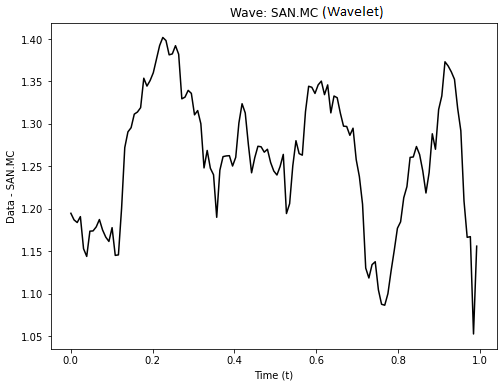
\includegraphics[width=.9\linewidth]{serie wavelet}
  \label{fig:sub2}
\end{subfigure}
\caption{Transformada Wavelet descartando los detalles}
\label{fig:test}
\end{figure}
			En nuestro caso es interesante ver si podemos desechar la serie que muestra los detalles y solamente quedarnos con la traza principal, si podemos conseguir hacer esto y se mantienen los resultados que se consiguen con la serie sin transformar hemos conseguido reducir el número de puntos a la mitad por cada vez que apliquemos la transformada.\\
\begin{figure}[H]
\centering
\begin{subfigure}{.3\textwidth}
  \centering
  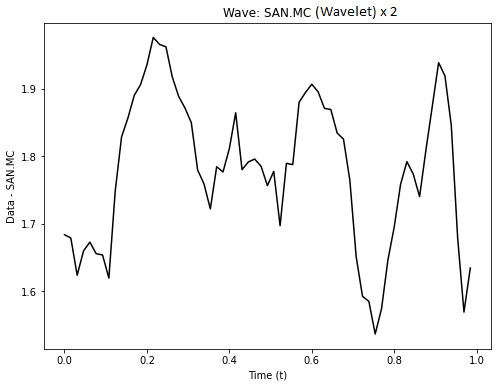
\includegraphics[width=.9\linewidth]{serie wavelet (1)}
  \label{fig:sub1}
\end{subfigure}%
\begin{subfigure}{.3\textwidth}
  \centering
  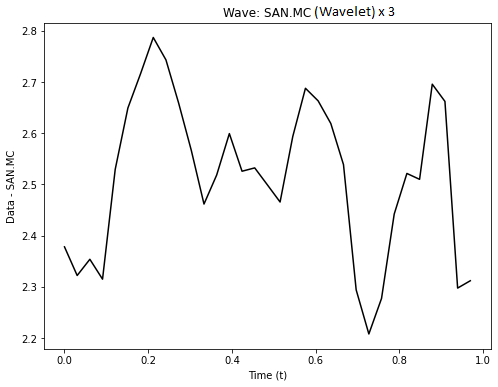
\includegraphics[width=.9\linewidth]{serie wavelet (2)}
  \label{fig:sub1}
\end{subfigure}%
\begin{subfigure}{.3\textwidth}
  \centering
  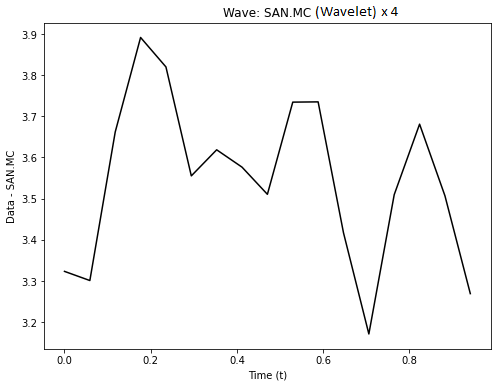
\includegraphics[width=.9\linewidth]{serie wavelet (3)}
  \label{fig:sub2}
\end{subfigure}
\caption{Transformada Wavelet aplicada 2/3/4 veces}
\label{fig:test}
\end{figure}
			Todo esto lo estudiaremos, y veremos si esta transformada o Fourier se adecuan a nuestro algoritmo, o si por el contrario ninguna mantiene una alta precisión con los resultados de las series sin transformar.
			\subsubsection{Grafo de Visibilidad}
			Esta transformación de la serie temporal es muy distinta a las dos anteriores, en este caso no buscamos optimizar el proceso manteniendo los resultados de la serie temporal sin transformar. Lo que buscamos aquí es conseguir resultados que tengan sentido pero que sean distintos a la serie sin transformar de esta forma tenemos dos caminos por donde ejecutar nuestro algoritmo y así poder compara los resultados obtenidos por cada camino.
			Pero antes de nada hay que explicar en que consiste la transformación a Grafo de Visibilidad. Como hemos dicho en los fundamentos teóricos es un proceso que crea un grafo a partir de una serie temporal, esto es muy útil porque nos permite tener un grafo con todas las propiedades y posibilidades que eso conlleva pero por medio de ese grafo seguir hablando de la serie temporal que lo genera permitiéndonos en nuestro caso clasificar esas series a través de propiedades de grafos.\\
\begin{figure}[H]
\centering
\begin{subfigure}{.3\textwidth}
  \centering
  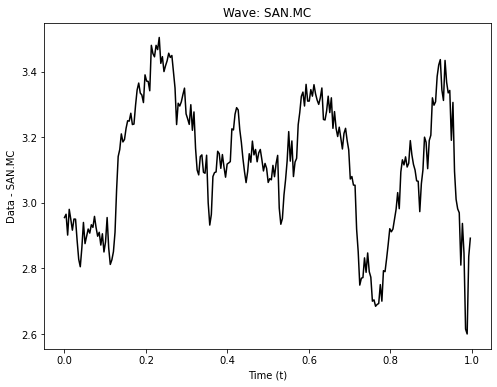
\includegraphics[width=.9\linewidth]{serie}
  \label{fig:sub1}
\end{subfigure}%
\begin{subfigure}{.3\textwidth}
  \centering
  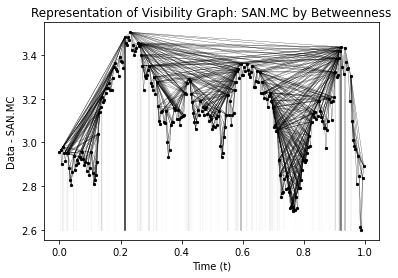
\includegraphics[width=.9\linewidth]{grafo de visibilidad (2)}
  \label{fig:sub1}
\end{subfigure}%
\begin{subfigure}{.3\textwidth}
  \centering
  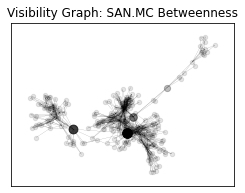
\includegraphics[width=.9\linewidth]{grafo de visibilidad (1)}
  \label{fig:sub2}
\end{subfigure}
\caption{Transformación de serie a grafo de visibilidad con la intensidad de los nodos proporcional a su centralidad betweenness}
\label{fig:test}
\end{figure}
			Esto tienes sus limitaciones ya que la transformación no es biyectiva así que no podemos asegurar recuperar nuestra serie una vez que tenemos el grafo. Esto se debe a que pequeñas perturbaciones en la serie no corresponden a pequeños cambios en el grafo.\\
			
			
		\subsection{Clusterización / K-means}
			\subsubsection{Razón de uso}
			La clusterización consiste en la agrupación de elementos mediante algún proceso consistente. En concreto k-means como hemos explicado en los fundamentos es un algoritmo que permite realizar esta clusterización de forma fácil y rápida, pero esa no es la razón principal por lo que lo vamos a utilizar. La mayor ventaja de k-means es la facilidad con la que se puede customizar, el algoritmo esta diseñado de tal forma que puede aceptar una gran diversidad de elementos. Lo único que se necesita es que se pueda definir una distancia entre los elementos que pasamos al algoritmo, si esto se cumple el algoritmo nos dará resultados.\\
			En nuestro caso la entrada son ondas temporales, las cuales a simple vista no parece que tengan una distancia definida entre ellas, pero si pensamos en la serie temporal como una serie de puntos ordenados podemos transformar este objeto bidimensional en un punto en un espacio N-dimensional cuya posición viene dada por el valor que toma en cada instante de tiempo.\\
\begin{figure}[H]
\centering
\begin{subfigure}{.5\textwidth}
  \centering
  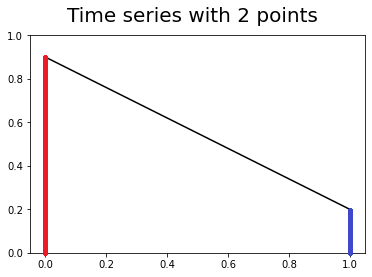
\includegraphics[width=.9\linewidth]{Ejemplo R2 (1)}
  \label{fig:sub1}
\end{subfigure}%
\begin{subfigure}{.5\textwidth}
  \centering
  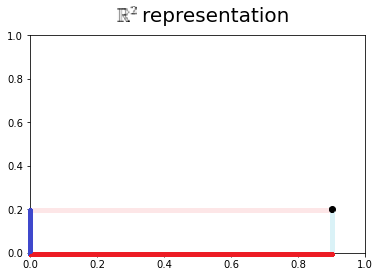
\includegraphics[width=.9\linewidth]{Ejemplo R2 (2)}
  \label{fig:sub2}
\end{subfigure}
\caption{Ejemplo de la conversión anteriormente escrita en $\mathbb{R}^2$}
\label{fig:test}
\end{figure}
Al estar los elementos de la serie equiespaciados temporalmente no necesitamos incluir el tiempo como una variable adicional en la representación.\\
			Este espacio N-dimensional tiene tantas dimensiones como valores tenga la serie a lo largo del tiempo, y como esos valores son reales el espacio en el que estamos es $R^n$ y en este espacio nuestros elementos son todos puntos por lo que estamos de suerte ya que $R^n$ es un espacio métrico y por lo tanto existen funciones distancia entre sus puntos. Con esto hemos podemos utilizar por defecto la distancia genérica en $R^n$ para realizar el algoritmo.\\
			
			\subsubsection{Customización}
			Como hemos dicho antes la customización es la herramienta más interesante que nos da k-means, esta customización se pude aplicar en dos partes diferentes.\\
			\textbf{Distancia}\\
			La distancia que se utiliza en el algoritmo solo tiene que ser valida entre los elementos de entrada por lo que vale cualquier distancia que sea formalmente correcta. Antes hemos mencionado la distancia genérica en $R^n$ como una posibilidad pero no es la única.\\
			Una distancia alternativa que vamos a tener en cuenta en nuestro estudio la vamos a llamar distancia rumbo que consiste en estudiar si la serie aumenta de valor o disminuye de valor en cada instante de tiempo, esta información en un principio se colapsaba en un valor único el cual posteriormente se trata como un punto unidimensional para comparar los elementos, este valor es producido de la siguiente forma:\\
			tengamos una serie $S$ y un intervalo temporal $(0,n)$
			\[rumbo_S =\sum_{i=0}^{n-1} x_i \]
			con
			\[x_i= \left\{ \begin{array}{lcc}
             1 &   si & S(t_i) < S(t_{i+1}) \\
             0.5 & si & S(t) = S(t_{i+1})\\
             0 &  si  & S(t_i) > S(t_{i+1})
             \end{array}
   			\right.
			\forall i \in (0,n-1)\]
			Pero al implementarla de esta forma me di cuenta de que de así se pierde información muy importante ya que solo me quedo con el valor correspondiente al numero total de subidas no se sabe en que momento se producen las subidas y bajadas de valor, así que al final opté por otro proceso que recogiera la misma idea. El nuevo proceso consiste en mantener el check de subidas y bajadas de valor, pero esta vez los resultados se quedan en forma de onda de la siguiente forma:\\
			\[rumbo_S(t)= \left\{ \begin{array}{lcc}
             1 &   si & S(t) < S(t+1) \\
			0.5 & si & S(t) = S(t+1)\\
             0 &  si  & S(t) >  S(t+1)
             \end{array}
   			\right.\]
\begin{figure}[H]
\centering
  \centering
  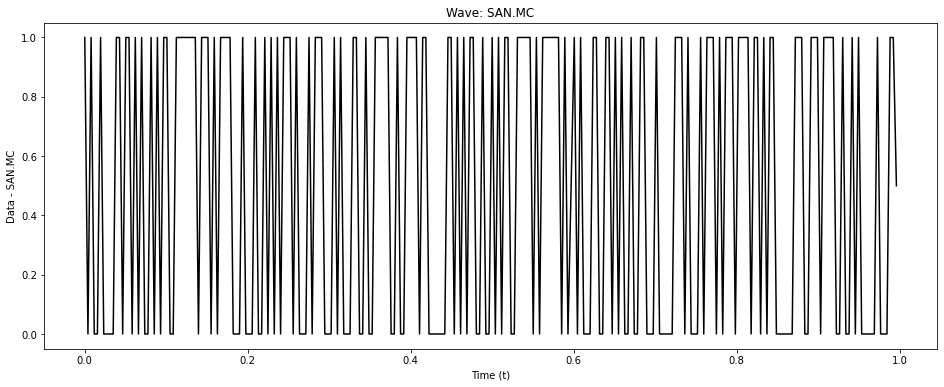
\includegraphics[width=1\linewidth]{course}
\caption{Serie resultante de aplicar la formula anterior a los datos del banco Santander ya mostrados}
\label{fig:test}
\end{figure}
			Y sobre esto se aplica la distancia genérica y de esta forma si que podemos mantener la información de donde están las subidas y bajadas.\\
			Un paso más allá de la distancia rumbo tenemos la distancia rumbo valor, en vez de solo fijarnos en la cantidad de subidas y bajadas podemos ademas recoger el valor de esa subida como podemos ver a continuación:\\
			\[rumboValor_S(t)= S(t+1) - S(t)\]
\begin{figure}[H]
\centering
  \centering
  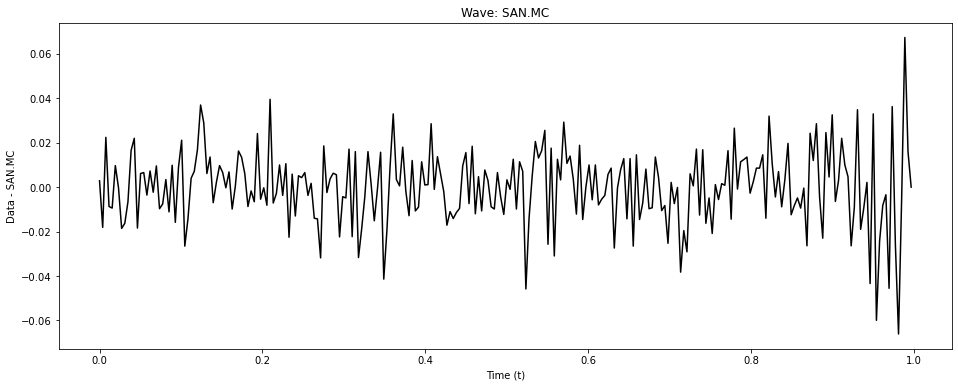
\includegraphics[width=1\linewidth]{course value}
\caption{Serie resultante de aplicar la formula anterior a los datos del banco Santander ya mostrados}
\label{fig:test}
\end{figure}
			Con esto cubrimos las distancias que vamos a utilizar en nuestro algoritmo, pero mi intuición me dice que de entre estas tres distancias la distancia rumbo va a darnos peores resultados que las otras dos ya que la distancia rumbo valor parece una mejora lógica de la otra distancia, pero todavía no puedo prever si esta distancia dará mejores resultados que la distancia genérica.\\
			\textbf{Inicialización de centroides}\\
			Como se inicializan los centroides es otra parte que permite customización aunque en este caso no es algo tan bueno ya que dependiendo de como se inicialicen los centroides los resultados del algoritmo pueden ser altamente distintos debido a las limitaciones que tiene k-means.\\
			En nuestro caso vamos a inicializar los k centroides de una forma bastante convencional que es asignando los k primeros elementos a los k centroides, es posible también hacerlo de otra forma, como por ejemplo selección aleatoria, pero en principio no existe una clara forma de elegir centroides que sea superior a las demás.
			En este proyecto vamos a intentar limitar la disparidad de los posibles resultados del algoritmo haciendo modificaciones sobre la propia estructura de k-means como vamos a mostrar a continuación.
			\subsection{K-means cíclico}
			
			(La conversión del input en nodos de un grafo con peso dependiente de las veces que están en el mismo cluster)
			\subsubsection{Motivación}
			En este apartado hablaremos de como modificar k-means para poder ejecutarlo en bucle lo cual conceptualmente es fácil de ver, pero es bastante más difícil de implementar.\\
			Nuestra motivación es mejorar la consistencia de los resultados del algoritmo repitiéndolo varias veces con distinta inicialización de centroides. En nuestro caso el número de repeticiones del algoritmo será igual al número de elementos de entrada, de esa forma tendremos una cantidad decente de repeticiones sin comprometer demasiado la eficiencia característica de k-means.\\
			La mayor dificultad para hacer factible el k-means cíclico reside en resolver como almacenar y transformar los resultados de cada iteración para poder al final tener clusteres, que es lo que se espera de este algoritmo. \\
			
			\subsubsection{Cambios}
			
			 Primero empecemos por la parte fácil, y lo fácil en este caso es hacer los cambios necesarios en cada iteración para que no estemos repitiendo lo mismo todo el rato. Para cambiar como se cogen los primeros centroides seguiremos cogiendo los k primeros elementos pero en cada iteración los desplazamos un elemento hacia delante para que al final del bucle todos los elementos hayan sido iniciadores de centroides.\\
			 Ahora vamos a hablar de como analizar los resultados, cuando k-means da como resultado que dos elementos están en el mismo cluster quiere decir que esos elementos están cerca, por lo tanto, si creamos para cada elemento una relación con los demás elementos que están en el mismo cluster hemos transformado toda la información que nos da cada iteración a un formato que si podemos expandir.\\
			 Aquí mostramos un ejemplo de este proceso:\\
\begin{figure}[H]
\centering
\begin{subfigure}{.5\textwidth}
  \centering
  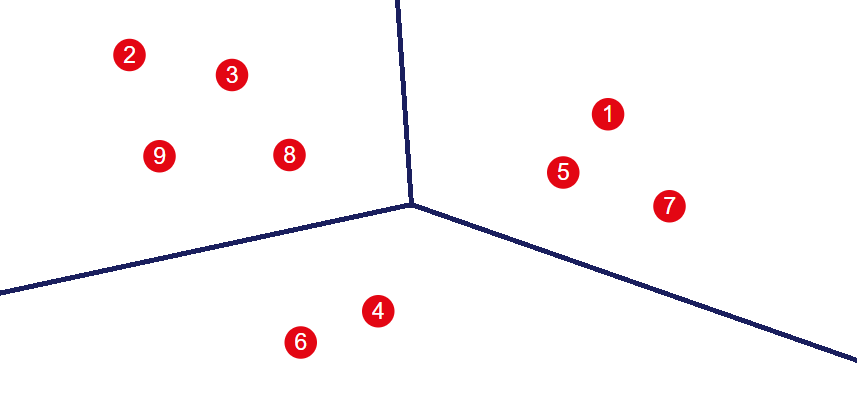
\includegraphics[width=.9\linewidth]{cluster 1}
  \label{fig:sub1}
\end{subfigure}%
\begin{subfigure}{.5\textwidth}
  \centering
  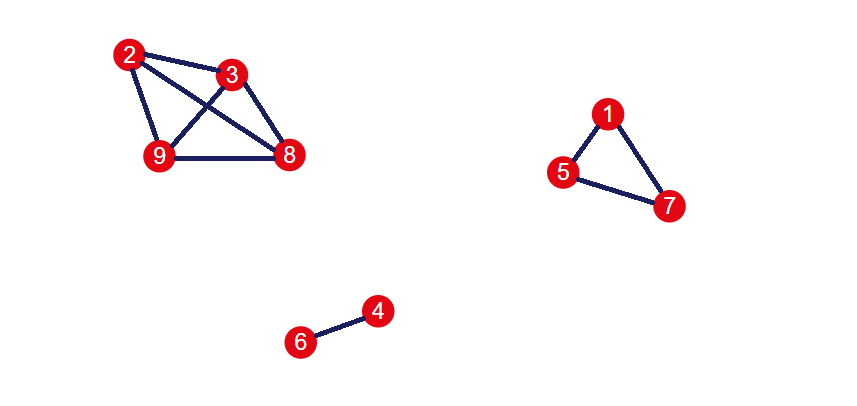
\includegraphics[width=.9\linewidth]{grafo cluster 1}
  \label{fig:sub2}
\end{subfigure}
\caption{1ª iteración, los cluster se transforman en conexiones}
\label{fig:test}
\end{figure}
\begin{figure}[H]
\centering
\begin{subfigure}{.5\textwidth}
  \centering
  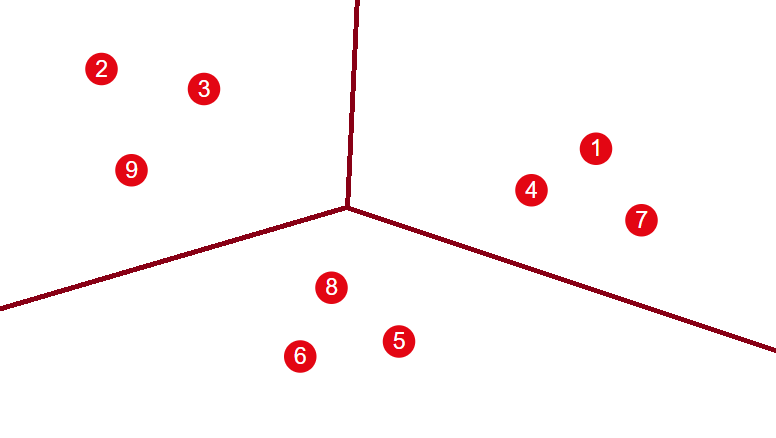
\includegraphics[width=.9\linewidth]{cluster 2}
  \label{fig:sub1}
\end{subfigure}%
\begin{subfigure}{.5\textwidth}
  \centering
  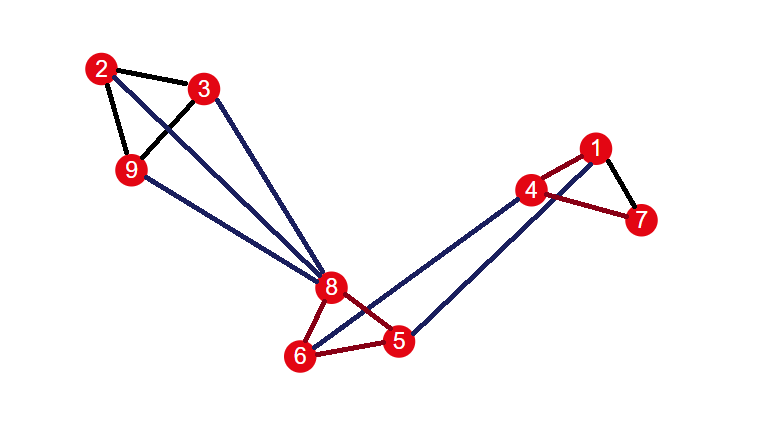
\includegraphics[width=.9\linewidth]{grafo cluster 2}
  \label{fig:sub2}
\end{subfigure}
\caption{2ª iteración, las aristas negras tienen peso 2, las aristas azules se mantienen de la iteración 1 y los las aristas granate son nuevas conexiones}
\label{fig:test}
\end{figure}
			 Con esto podemos trasladar los resultados de una lista de conjuntos con los elementos dentro a un grafo cuyos nodos son los elementos y el peso de sus aristas son el número de veces que los elementos conectados han estado en el mismo cluster, pero ese peso se tiene que invertir ya que a mayor número de veces que están dos elementos en el mismo cluster más cerca están y eso tenemos que reflejarlo en el grafo para poder hacer operaciones de grafos sobre el mismo.\\
\begin{figure}[H]
\centering
\begin{subfigure}{.5\textwidth}
  \centering
  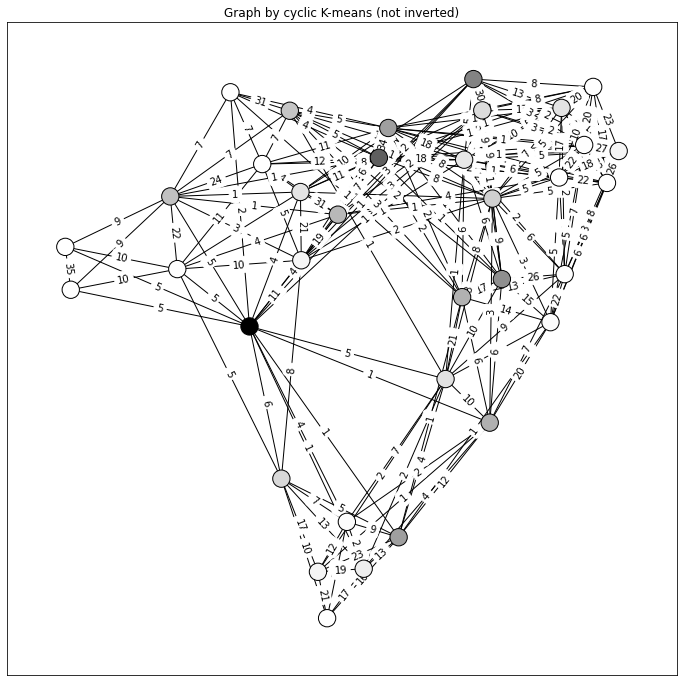
\includegraphics[width=.9\linewidth]{grafo kmeans ciclico}
  \caption{Peso corresponde al número de veces que dos nodos están en el mismo cluster}
  \label{fig:sub1}
\end{subfigure}%
\begin{subfigure}{.5\textwidth}
  \centering
  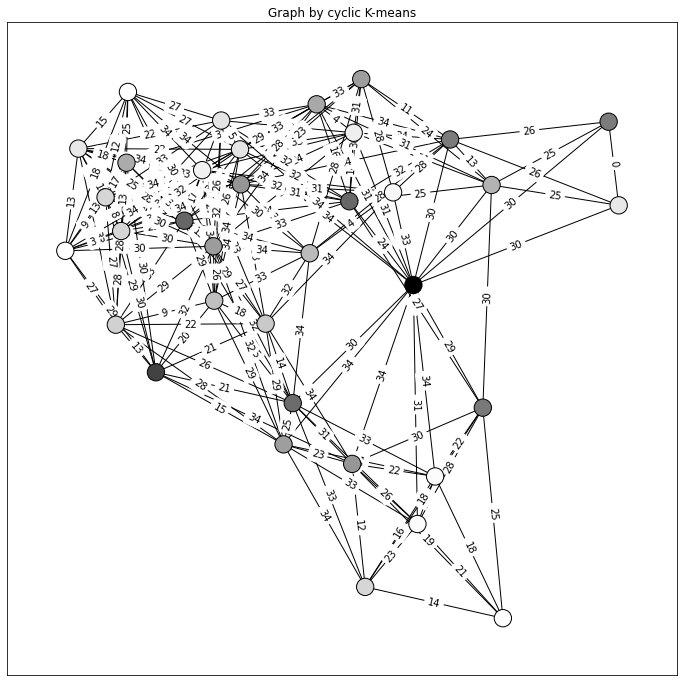
\includegraphics[width=.9\linewidth]{grafo kmeans ciclico invertido}
  \caption{Peso invertido\\ \phantom{filler}}
  \label{fig:sub2}
\end{subfigure}
\caption{Resultado del algoritmo K-means cíclico}
\label{fig:test}
\end{figure}
			 Todos estos cambios los denotamos en el siguiente pseudocódigo:\\
\begin{algorithm}[H]
			    \caption{K-means cíclico}\label{euclid}
			    \hspace*{\algorithmicindent} \textbf{Input: {\normalfont   Data} $\mathcal{X} = \{x_1..x_n\}$}\\
			    \textbf{\tab \tab {\normalfont \quad Numero de clusters}  ${k}$}\\
			    \textbf{\tab \tab {\normalfont \quad Valor umbral}  ${ \varepsilon }$}\\
			    \hspace*{\algorithmicindent} \textbf{Output:{\normalfont \quad Grafo} $G=(V,E)$} 
			    \begin{algorithmic}[1]
			    \Procedure{K-means cíclico}{$\mathcal{X},k,\varepsilon$}
			    \State \# \textit{Creamos un grafo para guardar los resultados en $\mathcal{K}$}
			    \State $G=(V,E)$
			    \State $G[V] \gets \mathcal{X}$ 
				\For{$x \in \mathcal{X}$} \do
				\State \State $\mathcal{X} \gets shuffle(\mathcal{X})$
				\State 	\# \textit{Llamada al algoritmo K-Means sin modificar}
				\begingroup
        			\color{blue}
				\State {$\mathcal{K} \gets KMeans (\mathcal{X},k,\varepsilon)$}
				\endgroup
				\State {$G[E] \gets clusterToGraph(\mathcal{K},G)$}
				
		            \EndFor
			    \BState \textbf{return} G;
			    \EndProcedure
			    \end{algorithmic}
			    \end{algorithm}
			  Y como podemos ver fácilmente la complejidad de este algoritmo es $\mathbf{O(n \cdot O_{k-means})}$\\
 			\subsubsection{Dificultades}
 			Un problema con el que nos hemos topado aquí es el decidir el número de iteraciones que realizar. Mi idea al principio era maximizar la precisión haciendo un bucle extra por encima de todo recorriendo cualquier posible número de clusters k de 1 a n, de forma que la complejidad del algoritmo se iba a $O(n^2 \cdot O_{k-means}))$ que no parece mucho pero en este punto ya se empezaba a notar.\\
 			Sin duda el mayor problema que tenemos con este algoritmo es que realmente no tenemos los resultados en el formato esperado, tenemos un grafo cuando esperábamos una lista de clusters. Ahora necesitamos hacer un análisis sobre este grafo para sacar los clusters y para eso necesitaremos el algoritmo que explicaremos a continuación.\\
			\subsection{K-means sobre grafos}
			\subsubsection{Motivación}
			Debido a los resultados del k-means cíclico hemos llegado a un grafo que todavía hay que clusterizar, esto lo podríamos hacer utilizando un método de clusterización especifico para grafos ( como puede ser el método de Girvan-Newman que utilicé en un principio)pero ya que hemos llegado hasta aquí con k-means resultaría interesante resolver este problema también con k-means. Por suerte nos podemos basar en \cite{Kmeans} para ello.\\
			 \begin{figure}[H]
\centering
  \centering
  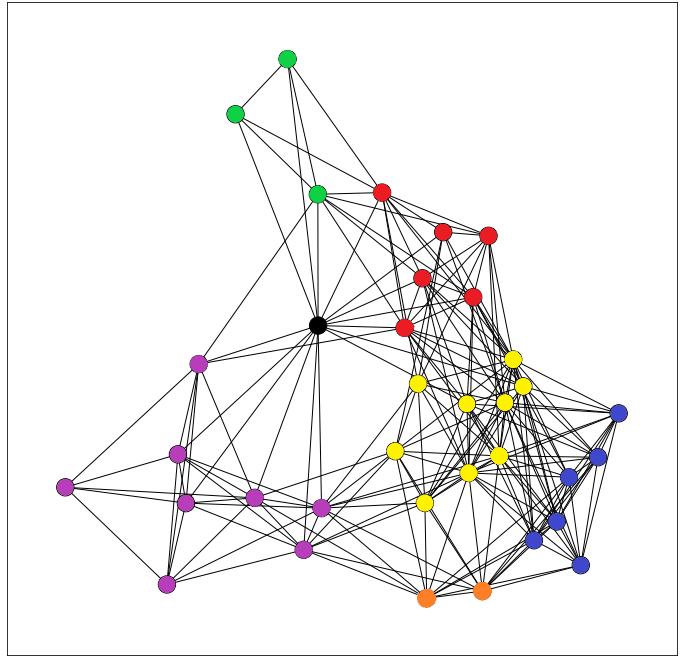
\includegraphics[width=1\linewidth]{kmeans ciclico clusters}
\caption{Grafo resultante de aplicar k-means cíclico sobre los valores del IBEX-35 separado en 7 clusters}
\label{fig:clusters}
\end{figure}
			
			\subsubsection{Cambios}
			Lo primero que hay que tener en cuenta es que un grafo restringe mucho la rectificación de centroides, en k-means convencionalmente al final de cada iteración se elige una nueva lista de centroides que se calculan haciendo el promedio de los elementos de cada cluster. El problema en un grafo es que hacer el promedio de elementos no tiene sentido ya que si lo piensas en un grafo no hay nada entre los nodos, no hay puntos intermedios que se puedan asignar como centroides.\\
			Esto solo lo podemos solucionar si restringimos los centroides a ser elegidos entre el conjunto de nodos, pero ahora tenemos que buscar otra forma de cambiar los centroides y para ello utilizaremos propiedades de los grafos.\\
			Como es de esperar para elegir el nuevo centroide de un cluster tenemos que fijarnos en los elementos que están dentro del cluster en esa iteración. Y aquí es donde nos ayuda tener un grafo, mientras que otros tipos de elementos no restan relacionados entre ellos como pueden ser las series temporales con las que empezamos, los un cluster de nodos de un grafo tienen sus aristas intactas convirtiendo virtualmente el cluster en un subgrafo del grafo completo.\\
			 \begin{figure}[H]
\centering
  \centering
  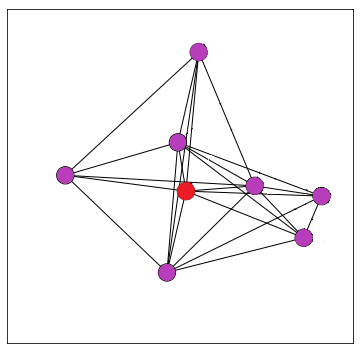
\includegraphics[width=0.5\linewidth]{subgrafo}
\caption{Subgrafo perteneciente  a la figura \ref{fig:clusters} resaltando su centroide en rojo }
\label{fig:subrgrafo}
\end{figure}
			
			Ahora bien, tenemos que recordar que lo que estamos buscando es sustituir el concepto de promedio por una aproximación para grafos y eso lo podemos hacer estudiando la centralidad de este subgrafo. Hay varios conceptos de centralidad que podemos utilizar como hemos mencionado anteriormente pero la mejor para este caso es la centralidad betweenness ya que es la que más se adecua para encontrar el nodo más cercano a todos los demás nodos que es básicamente lo que estamos buscando. Si utilizáramos por ejemplo la centralidad de grado tendríamos problemas al detectar cambios en el subgrafo si los nuevos nodos no se conectan directamente al nodo central.\\
			\begin{figure}[H]
\centering
\begin{subfigure}{.5\textwidth}
  \centering
  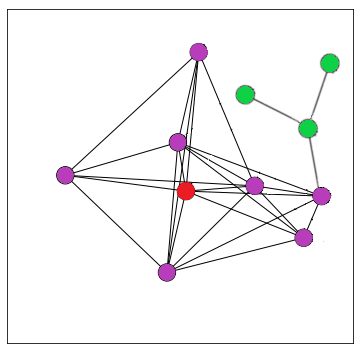
\includegraphics[width=.9\linewidth]{subgrafo nodos grado}
  \caption{Utilizando la centralidad de grado\\ el centroide no varia}
  \label{fig:sub1}
\end{subfigure}%
\begin{subfigure}{.5\textwidth}
  \centering
  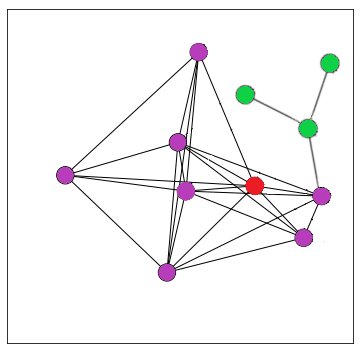
\includegraphics[width=.9\linewidth]{subgrafo nodos betweenness}
  \caption{Utilizando la centralidad betweenness el centroide varia}
  \label{fig:sub2}
\end{subfigure}
\caption{Extensión del subgrafo anterior}
\label{fig:test}
\end{figure}
			Cabe destacar que realmente estos cambios al algoritmo k-means realmente lo convierte en k medoids ya que los centroides solo pueden ser elegidos entre los nodos, pero como simplemente hemos partido de k-means y solo hemos añadido restricciones nos referiremos a este algoritmo como una modificación de k-means y no de k medoids. Y con estos cambios el algoritmo se queda así:\\
\begin{algorithm}[H]
			    \caption{K-means sobre grafo}\label{euclid}
			    \hspace*{\algorithmicindent} \textbf{Input: {\normalfont   Data} $G = (V,E)$}\\
			    \textbf{\tab \tab {\normalfont \quad Numero de clusters}  ${k}$}\\
			    \textbf{\tab \tab {\normalfont \quad Valor umbral}  ${ \varepsilon }$}\\
			    \hspace*{\algorithmicindent} \textbf{Output:{\normalfont \quad Clusters} $\mathcal{C}=\{C_1..C_k\}$} 
			    \begin{algorithmic}[1]
			    \Procedure{K-means sobre grafo}{$G,k,\varepsilon$}
			    
			    \State $exit = False$
			    \begingroup
        			\color{red}
			    \State $ \{\sigma_1..\sigma_k\}  \gets$ \textbf {InicializarCentroidesGrafo}($G,k$)
			    \endgroup
				\While{$exit == False$} \do
				\State \State $\mathcal{C}=\{C_1..C_k\} \gets \{\emptyset..\emptyset\}$
			    \State \# \textit{Distribución de elementos en clusters}
			    \State $C_i \gets \{x_j / d(\sigma_i,x_j)  \leq d(\sigma_h,x_j) \forall h  \in \{1..k\}  \}  \forall i  \in \{1..k\}$
			    \State \# \textit{Actualización de clusters con restricción para grafo}
			    \begingroup
        			\color{red}
			    \State $ \{new\sigma_1..new\sigma_k\}  \gets$ \textbf {ActualizarCentroidesGrafo}($G,k,\mathcal{C}$)
			    \endgroup
			    \State \# \textit{Comprobar la condición de parada}
			    \If {($ \sum_{i=1}^{k} d(\sigma_i,new\sigma_i) \leq  \varepsilon$)}
			    \State $exit \gets True$
			    \EndIf
			    \State $ \{\sigma_1..\sigma_k\}  \gets \{new\sigma_1..new\sigma_k\}$
		            \EndWhile
			    \BState \textbf{return} $\mathcal{C}$;
			    \EndProcedure
			    \end{algorithmic}
			    \end{algorithm}			
			    El algoritmo tiene complejidad $\mathbf{O( O_{k-means})}$ ya que aunque la inicialización de centroides es más compleja que con el algoritmo sin modificar(concretamente $n^2$ más compleja), está modificación esta fuera del bucle principal por lo que no aumenta la complejidad del algoritmo. La única modificación dentro de este bucle es la actualización de centroides que al solo ser una restricción de la actualización de centroides anterior no aumenta su complejidad computacional.\\
			\subsubsection{Dificultades / Limitaciones}
			Si mantenemos el algoritmo solo con los cambios anteriores llegamos a un k-means funcional, pero tenemos los mismo problemas de un k-means convencional que nos hace preguntarnos si realmente ha merecido la pena aumentar la complejidad del algoritmo con k-means cíclico y después k-means sobre el grafo, ya que lo único que hemos hecho es trasladar el problema de inicialización de centroides. Pero aquí viene un proceso que puede eliminar el problema por completo, gracias a estar en un grafo podemos inicializar los centroides de otra forma. Partiendo de un grafo $G=(V,E)$\\
			\[ centroide_1 = x \in V/ \forall y \in V betweeneess(x) > betweeneess(y) \]
			\[ centroide_i = x\in V/ \forall y \in V \sum_{n=1}^{i-1}d(n,x) > \sum_{n=1}^{i-1}d(n,y) \]
			Es decir, empezamos con el primer elemento que le elegimos como el nodo que tiene máxima betweenness, y como estamos en un grafo ahora podemos calcular fácilmente la distancia a los demás nodos con el algoritmo de dijkstra y elegimos el nodo más alejado, hacemos lo mismo ahora pero con dos nodos elegimos el más alejado de los dos por eso hacemos la suma de sus distancias y así tenemos una forma de inicializar centroides superior a la que utilizamos con el k-means convencional.\\
\pagebreak
\subsection{K-means con grafos como entrada}
			\subsubsection{Motivación}
			Una vez que hemos modificado k means para trabajar sobre un grafo nos interesa hacernos la pregunta ¿ Y si en vez de tener como elementos los nodos de un grafo tenemos grafos enteros?, esta pregunta viene dada por la introducción que hemos hecho a los grafos de visibilidad y como se pueden sacar de nuestras series temporales, en el momento no lo mencionamos, pero trabajar con grafos como elementos de entrada en k-means no parece posible, al fin y al cabo no hay forma de definir distancias entre dos grafos distintos, la misma cuestión parece no tener sentido. Pero por suerte no es la primera vez que han surgido estas preguntas, ya se han estudiado distintas distancias como la edit distance en \cite{DistGrafo} así que encontrar distancias entre grafos es posible. Como ya hemos visto antes los grafos tienen unas propiedades muy útiles que nos pueden servir en este caso buscar posibles distancias.\\
		Todo esto se remonta a la transformación a grafo de visibilidad que podemos aplicar a una serie temporal como vimos en la explicación del Input del algoritmo.	
\begin{figure}[H]
\centering
\begin{subfigure}{.5\textwidth}
  \centering
  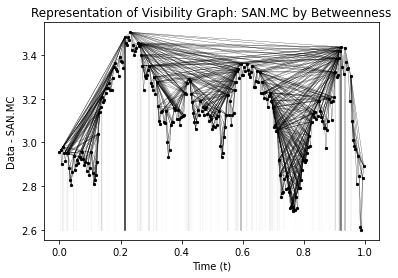
\includegraphics[width=.9\linewidth]{grafo de visibilidad (2)}
  \label{fig:sub1}
\end{subfigure}%
\begin{subfigure}{.5\textwidth}
  \centering
  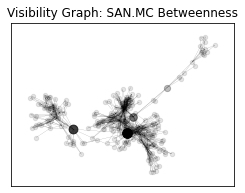
\includegraphics[width=.9\linewidth]{grafo de visibilidad (1)}
  \label{fig:sub2}
\end{subfigure}
\end{figure}
			
			\subsubsection{Centralidad}
			Necesitamos de alguna forma sacar de cada grafo una propiedad que pueda servir para ser comparada por lo que nos podemos basar a cuando nos surgió el mismo problema con las distancias rumbo. \\
			El primer enfoque es asignar a cada grafo un valor numérico fácilmente comparable como puede ser el máximo betweenness de los nodos de cada grafo, pero volvemos al problema de que perdemos mucha información.\\
			\[betweenness_G =max_{v\in V} betweenness(G[v]) \]
			El segundo enfoque es quedarse con la betweenness de todos los nodos y hacer K means sobre $R^n$, esto nos devuelve una serie de valores que por el momento es lo más complejo que sabemos procesas por k-means.\\
			\[\begin{array}{lcc}
S_G:G[V] \rightarrow \mathbb{R}\\
 \ \ \ \ \ \ \ \ \ \ \ v \rightarrow betweenness(v)
\end{array}\]
\begin{figure}[H]
\centering
  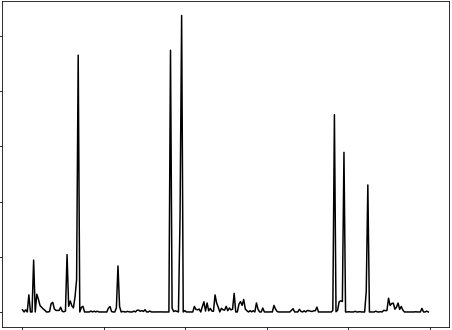
\includegraphics[width=.9\linewidth]{betweenness}
  \caption{Serie de valores betweenness del grafo de visibilidad}
\end{figure}
			\subsubsection{Dificultades / Limitaciones}
			El punto más tenso de este proceso es como se ha elegido betweenness como propiedad del grafo para compararlos. La otra posible propiedad que se ha barajado es la centralidad de grado pero esta propiedad tiene un gran problema, el valor de cada nodo solo depende de los nodos a los que esté conectado y en el grafo de visibilidad eso quiere decir que su valor solo depende de los nodos que ve directamente sin importar lo que les pase a los nodos que no ve. Este punto ciego en los datos que tiene la centralidad de grado ha hecho que nos decantemos por betweenness.\\
\pagebreak	
\subsection{Algoritmo completo}
	Hasta ahora hemos explicado todas las piezas necesarias para crear nuestro algoritmo. En este punto ya podemos exponer el algoritmo completo, y eso mismo vamos a hacer en el siguiente pseudocódigo.\\
\begin{algorithm}[H]
			    \caption{Selector de Stocks}\label{euclid}
			    \hspace*{\algorithmicindent} \textbf{Input: {\normalfont   Data} $\mathcal{X} = \{x_1..x_n\}$}\\
			    \textbf{\tab \tab {\normalfont \quad Numero de clusters}  ${k}$}\\
			    \textbf{\tab \tab {\normalfont \quad Valor umbral}  ${ \varepsilon }$}\\
			    \hspace*{\algorithmicindent} \textbf{Output:{\normalfont \quad Stocks} $\mathcal{S} = \{s_1..s_n\}$} 
			    \begin{algorithmic}[1]
			    \Procedure{Selector de Stocks}{$\mathcal{X},k,\varepsilon$}
			    \State \# \textit{Transformamos el input}
			    \begingroup
        			\color{red}
			    \State $\mathcal{X} \gets transformacion(\mathcal{X})$
			    \endgroup
			    \State $G=(V,E)$
			    	\begingroup
        			\color{blue}
			    \State $G \gets KMeansCiclico (\mathcal{X},k,\varepsilon)$ 
			    
			    \State $\mathcal{C} \gets KMeansGrafo(G,k,\varepsilon)$
			    \endgroup
				\State $\mathcal{S} = \{s_1..s_n\} \gets \{\emptyset..\emptyset\} $
				\For{$c \in \mathcal{C}$} \do
				\State \State	\# \textit{Selección del stocks que tenga menos volatilidad de cada cluster}
				\State  $\mathcal{S}.add(minVolatilidad(c)))$
		        \EndFor
			    \BState \textbf{return} $\mathcal{S}$;
			    \EndProcedure
			    \end{algorithmic}
			    \end{algorithm}
	De este pseudocódigo podemos calcular la complejidad computacional de nuestro algoritmo.\\
	La linea 2 tiene una complejidad variable ya que no siempre estamos aplicando la misma función, pero en el peor de los casos computacionalmente hablando le tenemos con la transformada a grafo de Visibilidad que nos da una complejidad $\mathbf{O(n \cdot t^3)}$ siendo n el número de stocks de entrada y t el intervalo temporal. \\
	La linea 5 consta de complejidad $\mathbf{O(n \cdot O_{k-means})}$\\
	La linea 6 consta de complejidad $\mathbf{O(O_{k-means})}$\\
	 El resto del algoritmo tiene complejidad $\mathbf{O(n\cdot t)}$ ya que el calculo de la volatilidad se realiza 1 vez por stock, y ese calculo tiene complejidad $\mathbf{O(t)}$.\\
	 En total: \[\mathbf{O(n \cdot t^3) + O(n \cdot O_{k-means}) + O(O_{k-means}) + O(n \cdot t) \\= O(max(n \cdot t^3,n \cdot O_{k-means})) }\]\\
	 En este caso nuestro O no es determinado, depende de la relación de n y t. Esto quiere decir que a veces la mayor parte del tiempo estará dedicada a hacer la transformación inicial y otras veces se le dedicará más tiempo al propio algoritmo.
\pagebreak


	\section{Experimentos / validación}
	
		\subsection{IBEX-35}
		El IBEX 35 es el principal indice de referencia de bolsa en España, está compuesto por las 35 empresas con más assets que cotizan en España en la actualidad. Esto tiene como positivo que asegura que las empresas que estudiamos están fuertemente establecidas lo que limita el riesgo de las inversiones. Lo negativo de esto es que como el IBEX 35 es dinámico, es decir las empresas que lo componen cambian, no podemos hacer un estudio exhaustivo del IBEX 35 sino que tendremos que hacer un estudio de las empresas que lo componen en un cierto instante de tiempo, nuestro estudio se basara en las empresas que están en el IBEX 35 en la actualidad.\\
		
		Estos datos aunque son completamente validos para este estudio tienen sus limitaciones ya que en comparación a otros indices de bolsa consta de pocas empresas. Por ejemplo tenemos el Standard \& Poor's 500 de Estados unidos que como su nombre indica tiene más de 500 empresas dentro. Pero como este proyecto se basa en el desarrollo de una nueva forma de análisis, hemos visto conveniente utilizar una entrada más pequeña de tan solo 35 empresas para facilitar el estudio.\\
		
		\subsection{Fourier vs Wavelet}
		Lo primero que conviene estudiar es la aplicación de las transformadas de Fourier y Wavelet para la optimización del algoritmo. En este contexto estamos buscando cual de los dos procesos distorsiona menos los resultados que nos da el algoritmo. Esto es difícil de comparar si ejecutamos el algoritmo entero ya que el algoritmo solo nos da una lista de elementos elegidos y no recoge información de como de cerca están esos elementos. Por lo tanto lo mejor es pararse a mitad del algoritmo justo antes de ejecutar el k-means sobre grafos, en ese punto tenemos un grafo con nodos relacionados por sus distancias concretas al ejecutar el k-means cíclico, en este punto hasta la variación más sutil puede ser medida.\\
		Ahora tenemos una meta clara, elegiremos la transformada que mantenga la mayor similitud entre los pesos de las aristas del grafo en comparación a las series sin transformar. Con esto dicho conviene calcular el porcentaje de error para tener una idea clara de cuanto se distorsionan los datos. Este error lo podemos calcular de la siguiente forma: \\
		\[ \%Error = \frac{error}{total} · 100\]
		con:\\
		
\[ total = \sum_{x \in E} \left | pesoReal(x) \right |\]
\[ error = \frac{1}{2}\sum_{x \in E} \left | pesoAprox(x)-pesoReal(x) \right |\]
		Conviene explicar de donde sale el $\frac{1}{2}$ en la ecuación del error. Si nos fijamos solo en el sumatorio el error se crea comparando el peso real con el peso aproximado, pero cada error produce 2 una diferencia de 2 ya que se contabiliza tanto la perdida de peso de la arista en la que estaba como la ganancia de peso de la arista en la que ahora está por lo tanto es necesario dividir entre dos el error.
		Si se prefiere se pude hablar de la precisión si lo calculamos como $\%Precision = 100 - \%Error$
		Con las formulas ya planteadas podemos hacer un estudio de Fourier en comparación a Wavelet. Para mejorar la precisión variaremos el intervalo de tiempo de los datos, los resultados están en la siguiente tabla:\\
\begin{table}[H]
\scalebox{0.72}{
\centering
\begin{tabular}{l|cc|cc|cc|cc|cc|cc|} 
\hline
\multicolumn{13}{c}{{\cellcolor[rgb]{0.635,0.647,0.788}}\%Precisión}                                                                                                                                                                                                                                                                                                                                                                                                                                                                                                                                                                                                                                                                                                                                                                                       \\ 
\hline
\rowcolor[rgb]{0.796,0.808,0.984} \multicolumn{1}{c|}{{\cellcolor[rgb]{0.635,0.647,0.788}}Año}                                                                                                & \multicolumn{2}{c|}{~ ~2016}                                                                            & \multicolumn{2}{c|}{2017~ ~}                                                                            & \multicolumn{2}{c|}{2018}                                                                               & \multicolumn{2}{c|}{2019}                                                                               & \multicolumn{2}{c|}{2020}                                                                               & \multicolumn{2}{c|}{2021}                                                                                \\ 
\hline
\rowcolor[rgb]{0.855,0.91,0.988} \multicolumn{1}{c|}{{\cellcolor[rgb]{0.635,0.647,0.788}}\begin{tabular}[c]{@{}>{\cellcolor[rgb]{0.635,0.647,0.788}}c@{}}Wavelet(W)\\Fourier(F)\end{tabular}} & W                                                  & {\cellcolor[rgb]{0.925,0.957,1}}F                  & W                                                  & {\cellcolor[rgb]{0.925,0.957,1}}F                  & W                                                  & {\cellcolor[rgb]{0.925,0.957,1}}F                  & W                                                  & {\cellcolor[rgb]{0.925,0.957,1}}F                  & W                                                  & {\cellcolor[rgb]{0.925,0.957,1}}F                  & W                                                  & {\cellcolor[rgb]{0.925,0.957,1}}F                   \\ 
\hline
\multicolumn{13}{c}{{\cellcolor[rgb]{0.796,0.808,0.984}}Algoritmo Estándar}                                                                                                                                                                                                                                                                                                                                                                                                                                                                                                                                                                                                                                                                                                                                                                                \\ 
\hline
\rowcolor[rgb]{0.925,0.957,1} Dist. genérica                                                                                                                                                  & \textbf{\textbf{\textcolor[rgb]{0,0.502,0}{85\%}}} & 28\%                                               & \textbf{\textbf{\textcolor[rgb]{0,0.502,0}{90\%}}} & 60\%                                               & \textbf{\textbf{\textcolor[rgb]{0,0.502,0}{89\%}}} & 41\%                                               & \textbf{\textbf{\textcolor[rgb]{0,0.502,0}{86\%}}} & 39\%                                               & \textbf{\textbf{\textcolor[rgb]{0,0.502,0}{87\%}}} & 58\%                                               & \textbf{\textbf{\textcolor[rgb]{0,0.502,0}{85\%}}} & 37\%                                                \\
\rowcolor[rgb]{0.855,0.91,0.988} Dist. rumbo                                                                                                                                                  & 55\%                                               & 43\%                                               & 45\%                                               & 40\%                                               & 53\%                                               & 48\%                                               & 54\%                                               & 37\%                                               & 48\%                                               & 45\%                                               & 56\%                                               & 41\%                                                \\
\rowcolor[rgb]{0.925,0.957,1} Dist. rumbo valor                                                                                                                                               & \textcolor[rgb]{0,0.502,0}{69\%}                   & 38\%                                               & \textcolor[rgb]{0,0.502,0}{69\%}                   & 43\%                                               & \textcolor[rgb]{0,0.502,0}{70\%}                   & 42\%                                               & \textcolor[rgb]{0,0.502,0}{72\%}                   & 41\%                                               & \textcolor[rgb]{0,0.502,0}{74\%}                   & 51\%                                               & \textcolor[rgb]{0,0.502,0}{84\%}                   & 41\%                                                \\ 
\hline
\multicolumn{13}{c}{{\cellcolor[rgb]{0.796,0.808,0.984}}Algoritmo Grafo~ ~ ~ ~ ~ ~ ~~}                                                                                                                                                                                                                                                                                                                                                                                                                                                                                                                                                                                                                                                                                                                                                                     \\ 
\hline
\rowcolor[rgb]{0.925,0.957,1} Dist. genérica                                                                                                                                                  & 9\%                                                & \textbf{\textbf{\textcolor[rgb]{0,0.502,0}{82\%}}} & 9\%                                                & \textbf{\textbf{\textcolor[rgb]{0,0.502,0}{88\%}}} & 14\%                                               & \textbf{\textbf{\textcolor[rgb]{0,0.502,0}{84\%}}} & 19\%                                               & \textbf{\textbf{\textcolor[rgb]{0,0.502,0}{83\%}}} & 30\%                                               & \textbf{\textbf{\textcolor[rgb]{0,0.502,0}{87\%}}} & 22\%                                               & \textbf{\textbf{\textcolor[rgb]{0,0.502,0}{85\%}}}  \\
\rowcolor[rgb]{0.855,0.91,0.988} Dist. rumbo                                                                                                                                                  & 45\%                                               & 36\%                                               & 44\%                                               & 42\%                                               & 40\%                                               & 36\%                                               & 30\%                                               & 22\%                                               & 33\%                                               & 18\%                                               & 34\%                                               & 33\%                                                \\
\rowcolor[rgb]{0.925,0.957,1} Dist. rumbo valor                                                                                                                                               & 11\%                                               & 20\%                                               & -11\%                                              & 23\%                                               & 1\%                                                & 21\%                                               & 0\%                                                & 27\%                                               & 9\%                                                & 19\%                                               & 0.5\%                                              & 30\%                                               
\end{tabular}}
\end{table}

		Como podemos ver en la tabla no hay duda hay dos resultados significativos. La transformada wavelet mantiene una alta precisión solamente en el caso por defecto sin la transformación a grafo de visibilidad lo cual nos es mucha sorpresa ya que la transformada wavelet mantiene a grandes rasgos la forma de la onda sin modificar, además la transformada wavelet también mantiene una precisión elevada al aplicar el algoritmo con la distancia rumbo valor para el proceso sin transformar a grafo, pero por desgracia los valores no son lo suficientemente y consistentemente altos para justificar su uso en este caso.\\
		Por otro lado tenemos a la transformada de fourier que por lo general se comporta peor que la transformada de fourier, pero sorprendentemente hay un caso especifico en el que supera de precisión a la transformada wavelet de forma consistente, y no solo eso, la precisión es suficientemente alta como para que aplicar la transformada en ese algoritmo sea factible, este caso es la distancia genérica cuando se aplica el grafo de visibilidad. Esto si nos paramos a pensarlo tiene sentido, el problema que tenia la transformada de fourier con las series sin transformar es que al estar compuestas por valores similares la transformada de fourier solo detecta una onda principal con máxima amplitud que eclipsa el resto de ondas que pueda detectar como vemos en la Figura 5, pero al aplicar la transformada a grafo de visibilidad y sacar la serie de centralidades los valores tienen mayor variación como se ve en la Figura 19, esto produce que la transformada de fourier detecte más ondas de amplitudes comparables lo que permite una mejor representación de la serie.\\
		Con este pequeño estudio podemos justificar el uso de estas transformadas en los casos que mantienen alta precisión.\\
		\subsection{Resultados}
		Casi llegamos al punto de comparar los resultados de nuestro algoritmo, lo único que nos queda es explicar qué es lo que realmente queremos conseguir.\\
		Estamos buscando como minimizar el riesgo en una inversión distribuida en partes iguales a k empresas que selecciona el algoritmo. Esta selección se hace una vez que se han clusterizado las empresas, en cada cluster se busca el mejor elemento según nuestro criterio, y ese criterio es el elemento de mínima volatilidad mediante la formula mostrada en los fundamentos teóricos y esto nos da k empresas en las que invertir para minimizar el riesgo según nuestro algoritmo (Veremos comparando los resultados con los métodos de control si esta meta se cumple).\\
		Uno se puede preguntar ¿que se consigue con esto? ¿ por que nos interesa minimizar la volatilidad y no maximizar ganancia?. Para empezar es cierto que estudiando todos los datos en un intervalo de tiempo es fácil ver como seleccionar una inversión que maximice las ganancias, pero por el simple hecho de tener a nuestra disposición estos datos quiere decir que el punto de poder invertir para conseguir esos resultados ya ha pasado, se podría invertir de esta forma esperando que las ganancias se mantengan, pero eso no se diferencia de invertir tirando los dados. Por eso utilizamos la volatilidad, nos aprovechamos de que el mercado en su conjunto tiende a subir para incrementar el valor de la inversión de forma consistente y lo que hace minimizar la volatilidad es limitar las perdidas y las ganancias ya que en ningún momento podemos estar seguros de que viene a continuación. La mejor parte de esto es que la volatilidad es una propiedad que tiende a mantenerse sin cambios bruscos a lo largo del tiempo por lo cual nos permite hacer estudios predictivos.\\
		En concreto vamos a utilizar la volatilidad ya explicada anteriormente pero delimitada a su equivalencia anual para que los valores de distintas simulaciones sean comparables. A esto lo llamamos volatilidad anual que básicamente consiste en dividir el valor de volatilidad entre los días del intervalo temporal y multiplicamos eso por 256 que son el número de valores que se recogen en 1 año. Lo que nos deja con la siguiente ecuación:
		\[VolatilidadAnual = {256}/{n}\sum_{i=1}^{n} \sqrt{\left | valor_i - media \right |} \]
		Con esto aclarado podemos empezar a analizar los datos.\\
		\subsubsection{Gráfico}
		El primer análisis consiste en los datos recogidos en un intervalo de 1 año (2021) con la selección de 4 empresas en las que invertir, esto son los valores que hemos puesto por defecto a nuestro algoritmo, esto resulta en la siguiente gráfica:\\
		{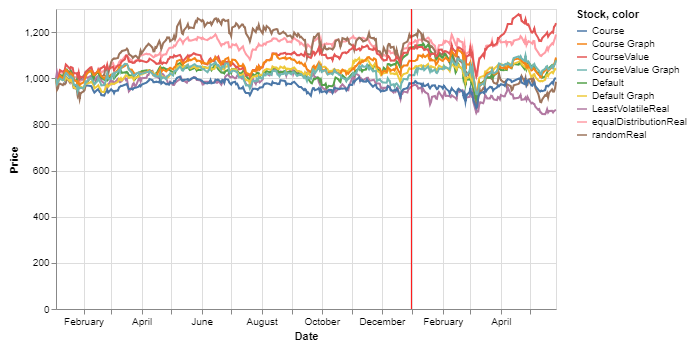
\includegraphics[scale=1]{results 1 year k=4}\par}
		Esta gráfica tiene todos los resultados superpuestos por lo que es un poco difícil visualizar los datos, pero esto no va ha ser un problema ya que vamos ha hacer un estudio numérico de los resultados. Pero de todas formas conviene explicar que representa cada parte.\\
		En el eje de abscisas tenemos representado el tiempo y la linea roja que lo corta separa el intervalo de tiempo que tenemos como input de los datos posteriores que no entran en el análisis.\\
		En el eje de ordenadas tenemos representado el valor económico de la inversión. Este proceso simula invertir 1000€ según lo que indica cada algoritmo y se ve la variación de valor de esa inversión inicial.\\
		Por último tenemos cada resultado representado en un color distinto como muestra la leyenda, vamos a ver estos resultados aislados a continuación:\\
		\begin{figure}[H]
    		\centering
    		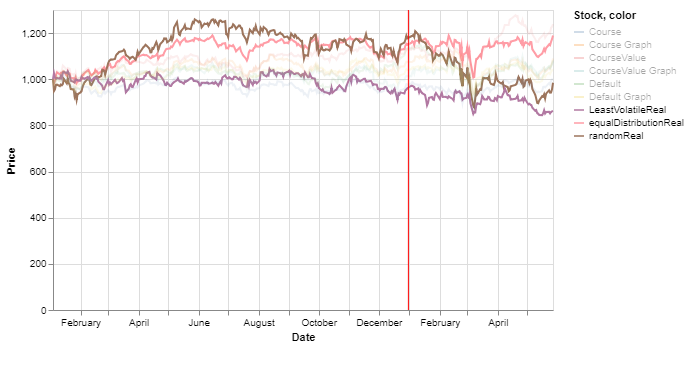
\includegraphics[scale=1]{results 1 year k=4 control}\par
    		\caption{Plot mostrando los valores de control}
		\end{figure}
		La imagen anterior muestra los 3 valores de control, inversión aleatoria en marrón, inversión homogénea en rosa e inversión todo a empresa con menos volatilidad en violeta.\\
		\begin{figure}[H]
    		\centering
    		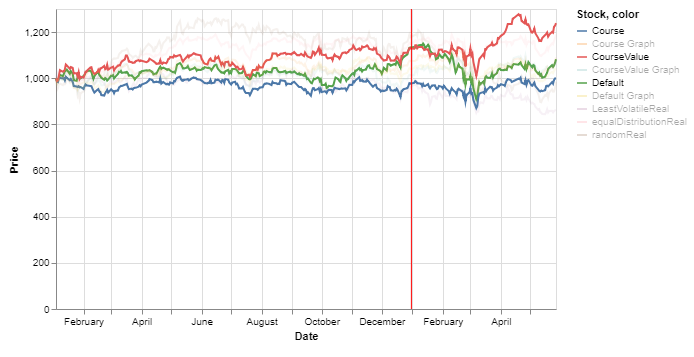
\includegraphics[scale=1]{results 1 year k=4 estandar}\par
    		\caption{Plot mostrando los resultados del k-means}
		\end{figure}
		La imagen anterior muestra los 3 resultados que nos da el algoritmo con el input sin transformar para las 3 distancias que acordamos antes, en verde esta representada la distancia genérica, en azul la distancia rumbo y en rojo la distancia rumbo valor.\\
		\begin{figure}[H]
    		\centering
    		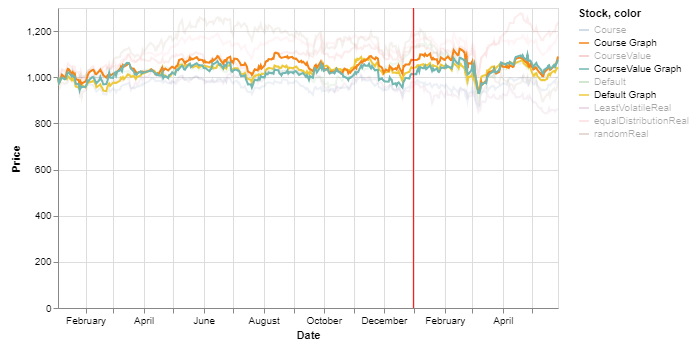
\includegraphics[scale=1]{results 1 year k=4 grafo}\par
    		\caption{Plot mostrando los resultados del k-means con grafos de visibilidad como input}
		\end{figure}
		Y por último esta imagen representa los resultados del algoritmo al hacer el grafo de visibilidad, en amarillo esta la distancia genérica, en naranja la distancia rumbo y en cian la distancia rumbo valor.\\
		\subsubsection{Tablas}
		La gráfica anterior muestra los siguientes datos hasta la linea roja.\\

\begin{table}[H]
\scalebox{0.66}{
\centering
\begin{tabular}{l|c|c|c|l|}
                                                     & Volatilidad & Valor   & \%Ganancias & \multicolumn{1}{c|}{Selección}       \\ 
\hline
\multicolumn{5}{c}{{\cellcolor[rgb]{0.796,0.808,0.984}}Control}                                                                   \\ 
\hline
\rowcolor[rgb]{0.925,0.957,1} Distribución Homogénea & 52.54       & 1149.57 & 14.9\%      & \multicolumn{1}{c|}{ALL}             \\
\rowcolor[rgb]{0.855,0.91,0.988} Random              & 82.49       & 1177.03 & 17.7\%      & ELE.MC / CIE.MC / IAG.MC / FDR.MC    \\
\rowcolor[rgb]{0.925,0.957,1} Min Volátil            & \color[HTML]{009901}25.31       & 960.78  & \color[HTML]{CB0000}-3.9\%      & \multicolumn{1}{c|}{VIS.MC}          \\ 
\hline
\multicolumn{5}{c}{{\cellcolor[rgb]{0.796,0.808,0.984}}Algoritmo Estándar}                                                        \\ 
\hline
\rowcolor[rgb]{0.925,0.957,1} Dist. genérica         & \color[HTML]{009901}25.7        & 1133.27 & 13.3\%      & NTGY.MC / ACS.MC / VIS.MC /CIE.MC    \\
\rowcolor[rgb]{0.855,0.91,0.988} Dist. rumbo         & \color[HTML]{009901}19.55       & 976.38  & \color[HTML]{CB0000}-2.4\%      & AENA.MC / IBE.MC / ENG.MC / VIS.MC   \\
\rowcolor[rgb]{0.925,0.957,1} Dist. rumbo valor      & 33.07       & 1128.79 & 12.8\%      & AENA.MC / ANA.MC / TEF.MC / VIS.MC   \\ 
\hline
\multicolumn{5}{c}{{\cellcolor[rgb]{0.796,0.808,0.984}}Algoritmo Grafo}                                                           \\ 
\hline
\rowcolor[rgb]{0.925,0.957,1} Dist. generica         & 29.93       & 1040.07 & 4\%         & AENA.MC / MAP.MC / VIS.MC / ENG.MC   \\
\rowcolor[rgb]{0.855,0.91,0.988} Dist. rumbo         & 28.64       & 1075.21 & 7.5\%       & CIE.MC / VIS.MC / AENA.MC / TEF.MC   \\
\rowcolor[rgb]{0.925,0.957,1} Dist. rumbo valor      & \color[HTML]{009901}26.19       & 1012.72 & 1.3\%       & TEF.MC / VIS.MC  / AENA.MC / AMS.MC 
\end{tabular}}
\end{table}
		
		Si ahora comparamos los datos de esta tabla con los nuevos valores que no recoge nuestro algoritmo tenemos lo siguiente:\\

\begin{table}[H]
\centering
\begin{tabular}{l|c|l|c|c|}
                                                     & Volatilidad                         & Dif Vol                             & Valor   & \%Ganancias                \\ 
\hline
\multicolumn{5}{c}{{\cellcolor[rgb]{0.796,0.808,0.984}}Control}                                                                                                         \\ 
\hline
\rowcolor[rgb]{0.925,0.957,1} Distribución Homogénea & 48.67                               & \textcolor[rgb]{0,0.6,0.004}{-3.87} & 1189.75 & 3.49\%                     \\
\rowcolor[rgb]{0.855,0.91,0.988} Random              & 98.35                               & \textcolor{red}{+15.86}             & 984.78  & \textcolor{red}{-16.33\%}  \\
\rowcolor[rgb]{0.925,0.957,1} Min Volátil            & 45.34                               & \textcolor{red}{+20.03}             & 862.75  & \textcolor{red}{-10.21\%}  \\ 
\hline
\multicolumn{5}{c}{{\cellcolor[rgb]{0.796,0.808,0.984}}Algoritmo Estándar}                                                                                              \\ 
\hline
\rowcolor[rgb]{0.925,0.957,1} Dist. genérica         & 36.64                               & +10.94                              & 1082.65 & \textcolor{red}{-4.47\%}   \\
\rowcolor[rgb]{0.855,0.91,0.988} Dist. rumbo         & \textcolor[rgb]{0,0.6,0.004}{21.29} & \textcolor[rgb]{0,0.6,0.004}{+1.74} & 1000.56 & 2.48\%                     \\
\rowcolor[rgb]{0.925,0.957,1} Dist. rumbo valor      & 53.69                               & \textcolor{red}{+20.62}             & 1238.57 & 9.7\%                      \\ 
\hline
\multicolumn{5}{c}{{\cellcolor[rgb]{0.796,0.808,0.984}}Algoritmo Grafo}                                                                                                 \\ 
\hline
\rowcolor[rgb]{0.925,0.957,1} Dist. generica         & \textcolor[rgb]{0,0.6,0.004}{29.72} & \textcolor[rgb]{0,0.6,0.004}{-0.21} & 1036.5  & \textcolor{red}{-0.34\%}   \\
\rowcolor[rgb]{0.855,0.91,0.988} Dist. rumbo         & 31.9                                & +3.26                               & 1089.45 & 1.33\%                     \\
\rowcolor[rgb]{0.925,0.957,1} Dist. rumbo valor      & \textcolor[rgb]{0,0.6,0.004}{30.23} & +4.04                               & 1077.54 & 6.4\%                     
\end{tabular}
\end{table}
		Solo con este pequeño estudio ya podemos notar que las ganancias no se pueden predecir, como ya se ha estudiado en \cite{Prediction}, así que de ahora en adelante ignoraremos las ganancias y nos centraremos en nuestro estudio de volatilidad,\\
		En este punto, antes de seguir con el estudio me gustaría exponer mi principal predicción sobre los datos.\\
		En primer lugar en comparación a los procesos de control (distribución homogénea, random y mínima volatilidad) los resultados van a ser mejores que la selección random ya que esta no sigue ningún criterio. Y los resultados van a ser peores que la distribución a mínima volatilidad ya que está diseñado para minimizar los parametros que se utilizan en la evaluación de los métodos. Por ultimo con relación a la distribución homogénea intuyo que los resultados van a ser equiparables ya que ambos métodos abordan el problema con el mismo enfoque, diversificar la inversión, la principal diferencia es como de extendida es la inversión.\\
A partir de ahora recurriremos a scripts para facilitar el proceso, tanto el (escrito en python) como los resultados están adjuntos como apéndices.\\
En la siguiente tabla tenemos los resultados promedios del algoritmo durante la totalidad del año 2021 eligiendo de 4 a 12 empresas del IBEX-35, y esto nos da los siguientes resultados
\begin{table}[H]
\centering
\begin{tabular}{l|c|l|c|} 
\hline
\multicolumn{4}{c}{{\cellcolor[rgb]{0.635,0.647,0.788}}Promedio 2021-01-01 / 2021-12-31}                                                                                            \\ 
\hline
\multicolumn{1}{c|}{{\cellcolor[rgb]{0.635,0.647,0.788}}k = 4~ . . 12} & Volatilidad                       & Dif Vol                           & Volatilidad Actual                 \\ 
\hline
\multicolumn{4}{c}{{\cellcolor[rgb]{0.796,0.808,0.984}}Control}                                                                                                                     \\ 
\hline
\rowcolor[rgb]{0.925,0.957,1} Distribución Homogénea                   & 52.54                             & -17,84                            & 34.7                               \\
\rowcolor[rgb]{0.855,0.91,0.988} Random                                & 53.23                             & -15.4                             & 37.83                              \\
\rowcolor[rgb]{0.925,0.957,1} Min Volátil                              & 25.31                             & +7.02                             & 32.33                              \\ 
\hline
\multicolumn{4}{c}{{\cellcolor[rgb]{0.796,0.808,0.984}}Algoritmo Estándar}                                                                                                          \\ 
\hline
\rowcolor[rgb]{0.925,0.957,1} Dist. genérica                           & 34.87                             & -2.36                             & 32.51                              \\
\rowcolor[rgb]{0.855,0.91,0.988} Dist. rumbo                           & 35.78                             & \textcolor{red}{-1.53}            & \textcolor{red}{34.25}             \\
\rowcolor[rgb]{0.925,0.957,1} Dist. rumbo valor                        & 32.27                             & -4.97                             & 27.3                               \\ 
\hline
\multicolumn{4}{c}{{\cellcolor[rgb]{0.796,0.808,0.984}}Algoritmo Grafo}                                                                                                             \\ 
\hline
\rowcolor[rgb]{0.925,0.957,1} Dist. generica                           & \textcolor{red}{38.15}            & \textcolor[rgb]{0,0.502,0}{-6.77} & 31.38                              \\
\rowcolor[rgb]{0.855,0.91,0.988} Dist. rumbo                           & 34.11                             & -5.38                             & 28.73                              \\
\rowcolor[rgb]{0.925,0.957,1} Dist. rumbo valor                        & \textcolor[rgb]{0,0.502,0}{28.19} & -3.38                             & \textcolor[rgb]{0,0.502,0}{24.72} 
\end{tabular}
\end{table}
	Aquí podemos ver que los resultados se mantienen consistentemente buenos durante la simulación pero necesitamos un sistema para cuantificar como de bueno es cada proceso en una simulación concreta para poder acumular los resultados con los de otras simulaciones. Lo que podemos hacer es crear un sistema de puntos con los que llevar la cuenta de que procesos dan mejores resultados a lo largo de varias simulaciones. Para esto nos resulta muy útil tener los datos de control como veremos a continuación\\
	Esto lo definimos de la siguiente forma:\\
	\begin{enumerate}
			\item Los datos de las tres columnas de cada proceso se comparan con los correspondientes datos de control y por cada uno que gane se le suma un punto al proceso.
			\item Además se otrogará un punto más por columna al mejor resultado, y se quitara un punto al peor.
	\end{enumerate}
	Esto ayuda a que cada simulación tenga el mismo peso en el resultado final, a diferencia de si utilizmos los numeros conretos de volatilidad con los cuales simulaciones con volatilidades generales distintas tendras distinto peso en el resultado.\\
	Para visualizar este proceso utilicemos como ejemplo la tabla anterior sustuyendo los valores por la puntuación.\\
	\begin{table}[H]
	
\centering
\begin{tabular}{l|c|l|c|c|} 
\hline
\multicolumn{5}{c}{{\cellcolor[rgb]{0.635,0.647,0.788}}Promedio 2021-01-01 / 2021-12-31}                                                                                                                               \\ 
\hline
\multicolumn{1}{c|}{{\cellcolor[rgb]{0.635,0.647,0.788}}k = 4~ . . 12} & Volatilidad                     & Dif Vol                         & Volatilidad Actual              & \multicolumn{1}{l|}{Total}              \\ 
\hline
\multicolumn{5}{c}{{\cellcolor[rgb]{0.796,0.808,0.984}}Control}                                                                                                                                                        \\ 
\hline
\rowcolor[rgb]{0.925,0.957,1} Distribución Homogénea                   & 52.54                           & -17,84                          & 34.7                            &                                         \\
\rowcolor[rgb]{0.855,0.91,0.988} Random                                & 53.23                           & -15.4                           & 37.83                           &                                         \\
\rowcolor[rgb]{0.925,0.957,1} Min Volátil                              & 25.31                           & +7.02                           & 32.33                           &                                         \\ 
\hline
\multicolumn{5}{c}{{\cellcolor[rgb]{0.796,0.808,0.984}}Algoritmo Estándar}                                                                                                                                             \\ 
\hline
\rowcolor[rgb]{0.925,0.957,1} Dist. genérica                           & 2                               & 1                               & 2                               & 5                                       \\
\rowcolor[rgb]{0.855,0.91,0.988} Dist. rumbo                           & 2                               & 1\textcolor{red}{-1}            & 2\textcolor{red}{-1}            & \textcolor{red}{\textbf{3}}             \\
\rowcolor[rgb]{0.925,0.957,1} Dist. rumbo valor                        & 2                               & 1                               & 3                               & 6                                       \\ 
\hline
\multicolumn{5}{c}{{\cellcolor[rgb]{0.796,0.808,0.984}}Algoritmo Grafo}                                                                                                                                                \\ 
\hline
\rowcolor[rgb]{0.925,0.957,1} Dist. generica                           & 2\textcolor{red}{-1}            & 1\textcolor[rgb]{0,0.502,0}{+1} & 3                               & 5                                       \\
\rowcolor[rgb]{0.855,0.91,0.988} Dist. rumbo                           & 2                               & 1                               & 3                               & 6                                       \\
\rowcolor[rgb]{0.925,0.957,1} Dist. rumbo valor                        & 2\textcolor[rgb]{0,0.502,0}{+1} & 1                               & 3\textcolor[rgb]{0,0.502,0}{+1} & \textcolor[rgb]{0,0.502,0}{\textbf{8}} 
\end{tabular}
\end{table}
De esta forma podemos acumular la puntuación a lo largo de varias simulaciones. Ahora mismo parece que el peor proceso es el estándar con la distancia rumbo, y el mejor el utilizando el grafo de visibilidad con la distancia rumbo valor, pero veamos si eso se mantiene.\\
Las tablas dedicadas al resto de simulaciones estarán en los apéndices, a continuación veremos los resultados de todas las simulaciones realizadas. Un total de de 8 simulaciones del promedio de resultados seleccionando de 4 a 12 empresas modificando el intervalo temporal.
\begin{figure}[H]
    		\centering
    		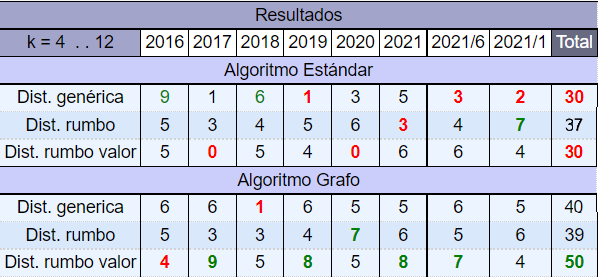
\includegraphics[scale=0.9]{Resultados}\par
    		\caption{Tabla con los resultados de simulaciones anuales de 2016 a 2021 , del primer mes de 2021 y de los primeros 6 meses de 2021}
		\end{figure}
		Antes de analizar los resultados cabe explicar el significado de las puntuaciones. Como las puntuaciones dependen de la comparación con los resultados de control, y sabemos que los resultados de control son, de mejor a peor, mínima volatilidad, distribución homogénea, y distribución random. Con esto podemos designar barreras a superar para que un proceso sea considerado mejor que los de control.\\

			\begin{enumerate}
			\item 		Si un proceso tiene 12 puntos es equivalente a la distribución random. Ya que como asumimos que la distribución random es la peor en los casos de control así que solo necesitamos una puntuación media de 1.5 a lo largo de las 8 simulaciones para ser equivalente.\\
			\item 		Si un proceso tiene 36 puntos es equivalente a la distribución homogénea. Asumimos que la distribución homogénea es mejor que la aleatoria así que hay que tener de media $3+1.5=4.5 (*8=36)$ puntos, 3 por ser consistemente mejor que random y 1.5 para comparase a la distribución homogénea.\\
			\item 		Si un proceso tiene 60 puntos es equivalente a la mínima volatilidad.Asumimos que la mínima volatilidad es la mejor porque esta diseñada para serlo y tenemos $3+3+1.5=7.5 (*8=60)$.\\

	\end{enumerate}	
		En la tabla de resultados se puede ver que hay una considerable diferencia entre los resultados, los procesos que se basan en en el grafo de visibilidad consiguen mejores resultados, y en concreto el proceso que además utiliza la distancia rumbo valor es la que nos ha dado los mejores resultados con diferencia.\\
		Con esta información podemos ejecutar nuestro algoritmo en un intervalo de tiempo que llegue hasta la actualidad y conforme nos diga este proceso en especifico hacer una recomendación de inversión dentro del IBEX-35.\\
	Ejecutando el caso que nos ha dado mejores resultados en el intervalo de tiempo 2016-01-01 hasta 2022-05-29 para que nos recomiende 4 empresas a invertir nos da como resultado ['MRL.MC', 'ELE.MC', 'REE.MC', 'NTGY.MC'], lo que quiere decir que recomienda invertir en Merlin Properties, Endesa, Red Electrica Corporación y Naturgy para minimizar el riesgo a futuro. (Esta simulación ha tardado 9 horas y media)
\pagebreak

	\section{Conclusiones}
	Durante todo el desarrollo de este proyecto se ha buscado encontrar una manera alternativa de diversificar una inversión en k empresas de forma comparable a otros métodos para minimizar el riesgo de dicha inversión. Esto se ha conseguido, y además se ha conseguido demostrar la utilidad del grafo de visibilidad para esta finalidad como una alternativa que parece mejorar todavía más los resultados de este algoritmo.\\
	En un principio la intención era crear un algoritmo que nos diese resultados comparables a la distribución homogénea, pero según las puntuaciones asignadas el algoritmo con el grafo de visibilidad ha sido consistentemente mejor que la distribución homogénea ya que en nuestro estudio una puntuación superior a 36 equivale a la distribución homogénea.\\
	Por otro lado nuestro estudio en busca de una transformada que nos permita optimizar el algoritmo no ha salido tan bien. Por un lado tenemos que descartar la transformada wavelet por completo ya que los dos casos en los que la transformada mantiene alta precisión son los dos casos en los que nuestro algoritmo da los peores resultados. Por otro lado tenemos la transformada de fourier que mantiene una alta precisión con la distancia genérica aplicada a la transformada en grafo que nos ha dado resultados mejores pero no ha sido el caso que mejores resultados nos ha dado. En definitiva la transformada de fourier es una mejor opción para optimizar el algoritmo, pero ninguna de las dos transformadas parecen ideales actualmente.
	
	Con esto dicho, todavía hay muchas posibles mejoras para el algoritmo bastante fáciles de afrontar que tienen la capacidad de mejorar todavía más los resultados:\\
	
	
	\begin{enumerate}
			\item La forma de seleccionar la empresa dentro de cada cluster es poco refinada ya que solo miramos su volatilidad, es posible que si tuviéramos en cuenta otros parámetros como la trayectoria del valor de la empresa pudiéramos mejorar los resultados.
			\item Ampliar el input utilizado para el estudio del IBEX-35 a un número mayor de empresas para asegurarnos que nuestros resultados no estén sesgados.
	\end{enumerate}	
	Por otro lado están las mejoras que son mucho más difíciles de afrontar:\\
	\begin{enumerate}
			\item Ahora mismo la inversión está distribuida en partes iguales para todas las empresas seleccionadas, pero es posible que permitir que la inversión no se reparta de forma homogénea entre todas las empresas mejoraría los resultados ya que eliminamos una restricción que nos limita las opciones. Desgraciadamente esto es algo que no es muy compatible con la estructura del algoritmo actualmente.
			\item Optimización general, ahora mismo las simulaciones anuales que nos han generado las tablas tardan alrededor de 40 minutos, y la ejecución para darnos la predicción ha tardado 9 horas y media, con estos tiempos no vendía mal optimizar el algoritmo, pero ahora mismo no parece haber muchas opciones en ese ámbito.
	\end{enumerate}	
\pagebreak

	\section{Bibliografía}
	 \renewcommand\refname{}
\begin{thebibliography}{X}


\bibitem{Kmeans} \textsc{Felipe Gonzalez Casabianca} \textsc{(2014)},
\textit{Algoritmos de Clustering en Grafos
Estáticos y Retos en Grafos Dinámicos}, \url{https://repositorio.uniandes.edu.co/bitstream/handle/1992/18461/u721646.pdf?sequence=1}

\bibitem{DistGrafo} \textsc{Gao, X., Xiao, B., Tao, D. et al. A survey of graph edit distance. Pattern Anal Applic 13, 113–129 (2010).} \url{https://doi.org/10.1007/s10044-008-0141-y}

\bibitem{Centalidad+} \textsc{ Pinar Sanz Sacristán}\textsc{(2018)},
\textit{ESTUDIO DE ALGORITMOS DE
COMPUTACIÓN BASADA EN
GRAFOS APLICADO AL
ANÁLISIS DE REDES
}, \url{https://repositorio.uam.es/bitstream/handle/10486/688032/sanz_sacrist%C3%A1n_pinar_tfg.pdf?sequence=1&isAllowed=y}

\bibitem{ComplejidadNP} \textsc{Ricardo Rosenfeld y Jerónimo Irazábal} \textsc{(2013)},
\textit{Computabilidad, complejidad
computacional y verificación
de programas}, \url{http://190.57.147.202:90/jspui/bitstream/123456789/988/1/computabilidad-complejidad-verificacion.pdf}

\bibitem{Clusters} \textsc{Magdalena Ferrán Aranaz} \textsc{(2011)},
\textit{UNA METODOLOGÍA DE MINERÍA DE DATOS
PARA LA AGRUPACIÓN DE SERIES
TEMPORALES: APLICACIÓN AL SECTOR DE LA
CONSTRUCCIÓN RESIDENCIAL. 
}, \url{https://eprints.ucm.es/id/eprint/12804/1/T32968.pdf}

\bibitem{Centralidad} \textsc{Regino Criado, Miguel Romance y Luis E. Solá} \textsc{(2014)},
\textit{Teoría de Perron-Frobenius:
importancia, poder y centralidad}, \url{https://gaceta.rsme.es/abrir.php?id=1217}

\bibitem{GrafoVisibilidadHorizontal} \textsc{Keshi Liu, Tongfeng Weng, Changgui Gu, Huijie Yang,
Visibility graph analysis of Bitcoin price series,
Physica A: Statistical Mechanics and its Applications,
Volume 538,
2020,
122952,
ISSN 0378-4371,}
\url{https://doi.org/10.1016/j.physa.2019.122952}

\bibitem{GrafoVisibilidad} \textsc{Lacasa, Lucas \& Luque, Bartolo \& Ballesteros, Fernando \& Luque, Jordi \& Nuño, Juan Carlos. (2008). From time series to complex networks: The visibility graph. Proceedings of the National Academy of Sciences. 105. 4972. 10.1073/pnas.0709247105.}

\bibitem{Wavelet} \textsc{Agbinya, Johnson. (1996). Discrete wavelet transform techniques in speech processing. 514 - 519 vol.2. 10.1109/TENCON.1996.608394. }

\bibitem{Fourier} \textsc{D. Song, A. M. Chung Baek and N. Kim, "Forecasting Stock Market Indices Using Padding-Based Fourier Transform Denoising and Time Series Deep Learning Models," in IEEE Access, vol. 9, pp. 83786-83796, 2021, doi: 10.1109/ACCESS.2021.3086537.}

\bibitem{Prediction} \textsc{S. M. Idrees, M. A. Alam and P. Agarwal, "A Prediction Approach for Stock Market Volatility Based on Time Series Data," in IEEE Access, vol. 7, pp. 17287-17298, 2019, doi: 10.1109/ACCESS.2019.2895252.}

\bibitem{Volatilidad} \textsc{CORREDOR, PILAR, SANTAMARÍA, RAFAEL PREDICCIÓN DE VOLATILIDAD Y PRECIOS DE LAS OPCIONES EN EL IBEX-35. Revista de Economía Aplicada [en linea]. 2001, IX(25), 39-64[fecha de Consulta 8 de Junio de 2022]. ISSN: 1133-455X. Disponible en: https://www.redalyc.org/articulo.oa?id=96917680002}

\bibitem{Complejidad} \textsc{Regino Criado Herrero, Roberto Muñoz Izquierdo} \textsc{(2007)},
\textit{Un semestre de matemática discreta
}

\end{thebibliography}

\pagebreak

	\section{Apéndices}
	\subsection{Script Wavelet vs Fourier}
\pythonexternal{code/scriptWavePrecision.py}
	\subsection{Script Volatilidad}
\pythonexternal{code/script.py}
	\subsection{Tablas de Promedios}
\begin{table}[H]
\centering
\begin{tabular}{l|c|l|c|} 
\hline
\multicolumn{4}{c}{{\cellcolor[rgb]{0.635,0.647,0.788}}Promedio 2016-01-01 / 2016-12-31}                                                                                             \\ 
\hline
\multicolumn{1}{c|}{{\cellcolor[rgb]{0.635,0.647,0.788}}k = 4~ . . 12} & Volatilidad                       & Dif Vol                            & Volatilidad Actual                 \\ 
\hline
\multicolumn{4}{c}{{\cellcolor[rgb]{0.796,0.808,0.984}}Control}                                                                                                                      \\ 
\hline
\rowcolor[rgb]{0.925,0.957,1} Distribución Homogénea                   & 45.88                             & -16.75                             & 29.13                              \\
\rowcolor[rgb]{0.855,0.91,0.988} Random                                & 69.86                             & -22.11                             & 47.75                              \\
\rowcolor[rgb]{0.925,0.957,1} Min Volátil                              & 31.42                             & +15.33                             & 46.75                              \\ 
\hline
\multicolumn{4}{c}{{\cellcolor[rgb]{0.796,0.808,0.984}}Algoritmo Estándar}                                                                                                           \\ 
\hline
\rowcolor[rgb]{0.925,0.957,1} Dist. genérica                           & 31.2                              & \textcolor[rgb]{0,0.502,0}{-12.73} & \textcolor[rgb]{0,0.502,0}{18.47}  \\
\rowcolor[rgb]{0.855,0.91,0.988} Dist. rumbo                           & 34.32                             & +1.43                              & 35.75                              \\
\rowcolor[rgb]{0.925,0.957,1} Dist. rumbo valor                        & 39.73                             & -5.95                              & 33.78                              \\ 
\hline
\multicolumn{4}{c}{{\cellcolor[rgb]{0.796,0.808,0.984}}Algoritmo Grafo}                                                                                                              \\ 
\hline
\rowcolor[rgb]{0.925,0.957,1} Dist. generica                           & 37.76                             & -8.96                              & 28.8                               \\
\rowcolor[rgb]{0.855,0.91,0.988} Dist. rumbo                           & \textcolor[rgb]{0,0.502,0}{29.16} & \textcolor{red}{+12.72}            & \textcolor{red}{41.88}             \\
\rowcolor[rgb]{0.925,0.957,1} Dist. rumbo valor                        & \textcolor{red}{42.93}            & -3.38                              & 39.55                             
\end{tabular}
\end{table}
	
\begin{table}[H]
\centering
\begin{tabular}{l|c|l|c|} 
\hline
\multicolumn{4}{c}{{\cellcolor[rgb]{0.635,0.647,0.788}}Promedio 2017-01-01 / 2017-12-31}                                                                                            \\ 
\hline
\multicolumn{1}{c|}{{\cellcolor[rgb]{0.635,0.647,0.788}}k = 4~ . . 12} & Volatilidad                      & Dif Vol                            & Volatilidad Actual                 \\ 
\hline
\multicolumn{4}{c}{{\cellcolor[rgb]{0.796,0.808,0.984}}Control}                                                                                                                     \\ 
\hline
\rowcolor[rgb]{0.925,0.957,1} Distribución Homogénea                   & 52.35                            & -27.25                             & 25.1                               \\
\rowcolor[rgb]{0.855,0.91,0.988} Random                                & 82.04                            & -27.84                             & 54.2                               \\
\rowcolor[rgb]{0.925,0.957,1} Min Volátil                              & 38.1                             & -19.38                             & 18.72                              \\ 
\hline
\multicolumn{4}{c}{{\cellcolor[rgb]{0.796,0.808,0.984}}Algoritmo Estándar}                                                                                                          \\ 
\hline
\rowcolor[rgb]{0.925,0.957,1} Dist. genérica                           & 50.17                            & \textcolor{red}{-11.25}            & 38.92                              \\
\rowcolor[rgb]{0.855,0.91,0.988} Dist. rumbo                           & 44.57                            & -15.81                             & 28.76                              \\
\rowcolor[rgb]{0.925,0.957,1} Dist. rumbo valor                        & \textcolor{red}{55.01}           & -15.61                             & \textcolor{red}{39.4}              \\ 
\hline
\multicolumn{4}{c}{{\cellcolor[rgb]{0.796,0.808,0.984}}Algoritmo Grafo}                                                                                                             \\ 
\hline
\rowcolor[rgb]{0.925,0.957,1} Dist. generica                           & 42.99                            & \textcolor[rgb]{0,0.502,0}{-22.86} & 20.13                              \\
\rowcolor[rgb]{0.855,0.91,0.988} Dist. rumbo                           & 46.87                            & -15.82                             & 31.05                              \\
\rowcolor[rgb]{0.925,0.957,1} Dist. rumbo valor                        & \textcolor[rgb]{0,0.502,0}{37.0} & -20.89                             & \textcolor[rgb]{0,0.502,0}{16.11} 
\end{tabular}
\end{table}
	
\begin{table}[H]
\centering
\begin{tabular}{l|c|l|c|} 
\hline
\multicolumn{4}{c}{{\cellcolor[rgb]{0.635,0.647,0.788}}Promedio 2018-01-01 / 2018-12-31}                                                                                             \\ 
\hline
\multicolumn{1}{c|}{{\cellcolor[rgb]{0.635,0.647,0.788}}k = 4~ . . 12} & Volatilidad                       & Dif Vol                            & Volatilidad Actual                 \\ 
\hline
\multicolumn{4}{c}{{\cellcolor[rgb]{0.796,0.808,0.984}}Control}                                                                                                                      \\ 
\hline
\rowcolor[rgb]{0.925,0.957,1} Distribución Homogénea                   & 35.15                             & -12.68                             & 22.47                              \\
\rowcolor[rgb]{0.855,0.91,0.988} Random                                & 44.37                             & -8.74                              & 35.63                              \\
\rowcolor[rgb]{0.925,0.957,1} Min Volátil                              & 31.53                             & +7.97                              & 39.5                               \\ 
\hline
\multicolumn{4}{c}{{\cellcolor[rgb]{0.796,0.808,0.984}}Algoritmo Estándar}                                                                                                           \\ 
\hline
\rowcolor[rgb]{0.925,0.957,1} Dist. genérica                           & \textcolor{red}{53.17}            & \textcolor[rgb]{0,0.502,0}{-18.73} & \textcolor[rgb]{0,0.502,0}{34.44}  \\
\rowcolor[rgb]{0.855,0.91,0.988} Dist. rumbo                           & \textcolor[rgb]{0,0.502,0}{27.64} & +19.53                             & 47.17                              \\
\rowcolor[rgb]{0.925,0.957,1} Dist. rumbo valor                        & 30.66                             & +7.18                              & 37.84                              \\ 
\hline
\multicolumn{4}{c}{{\cellcolor[rgb]{0.796,0.808,0.984}}Algoritmo Grafo}                                                                                                              \\ 
\hline
\rowcolor[rgb]{0.925,0.957,1} Dist. generica                           & 27.93                             & \textcolor{red}{+25.7}             & \textcolor{red}{53.63}             \\
\rowcolor[rgb]{0.855,0.91,0.988} Dist. rumbo                           & 28.11                             & +22.81                             & 50.92                              \\
\rowcolor[rgb]{0.925,0.957,1} Dist. rumbo valor                        & 30.63                             & +6.06                              & 36.69                             
\end{tabular}
\end{table}	
	
\begin{table}[H]
\centering
\begin{tabular}{l|c|l|c|} 
\hline
\multicolumn{4}{c}{{\cellcolor[rgb]{0.635,0.647,0.788}}Promedio 2019-01-01 / 2019-12-31}                                                                                            \\ 
\hline
\multicolumn{1}{c|}{{\cellcolor[rgb]{0.635,0.647,0.788}}k = 4~ . . 12} & Volatilidad                       & Dif Vol                           & Volatilidad Actual                 \\ 
\hline
\multicolumn{4}{c}{{\cellcolor[rgb]{0.796,0.808,0.984}}Control}                                                                                                                     \\ 
\hline
\rowcolor[rgb]{0.925,0.957,1} Distribución Homogénea                   & 40.55                             & -2.68                             & 37.87                              \\
\rowcolor[rgb]{0.855,0.91,0.988} Random                                & 46.85                             & -3.08                             & 43.77                              \\
\rowcolor[rgb]{0.925,0.957,1} Min Volátil                              & 44.3                              & +6.54                             & 50.81                              \\ 
\hline
\multicolumn{4}{c}{{\cellcolor[rgb]{0.796,0.808,0.984}}Algoritmo Estándar}                                                                                                          \\ 
\hline
\rowcolor[rgb]{0.925,0.957,1} Dist. genérica                           & \textcolor{red}{52.18}            & \textcolor[rgb]{0,0.502,0}{+2.93} & \textcolor{red}{55.11}             \\
\rowcolor[rgb]{0.855,0.91,0.988} Dist. rumbo                           & 30.36                             & +10.01                            & 40.37                              \\
\rowcolor[rgb]{0.925,0.957,1} Dist. rumbo valor                        & 31.23                             & \textcolor{red}{+10.57}           & 41.8                               \\ 
\hline
\multicolumn{4}{c}{{\cellcolor[rgb]{0.796,0.808,0.984}}Algoritmo Grafo}                                                                                                             \\ 
\hline
\rowcolor[rgb]{0.925,0.957,1} Dist. generica                           & 36.59                             & +3.15                             & 39.74                              \\
\rowcolor[rgb]{0.855,0.91,0.988} Dist. rumbo                           & 40.71                             & +4.28                             & 44.99                              \\
\rowcolor[rgb]{0.925,0.957,1} Dist. rumbo valor                        & \textcolor[rgb]{0,0.502,0}{25.38} & +7.57                             & \textcolor[rgb]{0,0.502,0}{32.95} 
\end{tabular}
\end{table}

\begin{table}[H]
\centering
\begin{tabular}{l|c|l|c|} 
\hline
\multicolumn{4}{c}{{\cellcolor[rgb]{0.635,0.647,0.788}}Promedio 2020-01-01 / 2020-12-31}                                                                                             \\ 
\hline
\multicolumn{1}{c|}{{\cellcolor[rgb]{0.635,0.647,0.788}}k = 4~ . . 12} & Volatilidad                       & Dif Vol                            & Volatilidad Actual                 \\ 
\hline
\multicolumn{4}{c}{{\cellcolor[rgb]{0.796,0.808,0.984}}Control}                                                                                                                      \\ 
\hline
\rowcolor[rgb]{0.925,0.957,1} Distribución Homogénea                   & 90.89                             & -43.2                              & 47.69                              \\
\rowcolor[rgb]{0.855,0.91,0.988} Random                                & 101.65                            & -39.35                             & 62.3                               \\
\rowcolor[rgb]{0.925,0.957,1} Min Volátil                              & 53.35                             & -24.01                             & 29.34                              \\ 
\hline
\multicolumn{4}{c}{{\cellcolor[rgb]{0.796,0.808,0.984}}Algoritmo Estándar}                                                                                                           \\ 
\hline
\rowcolor[rgb]{0.925,0.957,1} Dist. genérica                           & \textcolor{red}{90.19}            & -29.89                             & 60.3                               \\
\rowcolor[rgb]{0.855,0.91,0.988} Dist. rumbo                           & \textcolor[rgb]{0,0.502,0}{60.32} & -20.01                             & 40.31                              \\
\rowcolor[rgb]{0.925,0.957,1} Dist. rumbo valor                        & 88.61                             & \textcolor{red}{-19.59}            & \textcolor{red}{69.02}             \\ 
\hline
\multicolumn{4}{c}{{\cellcolor[rgb]{0.796,0.808,0.984}}Algoritmo Grafo}                                                                                                              \\ 
\hline
\rowcolor[rgb]{0.925,0.957,1} Dist. generica                           & 69.35                             & -31.63                             & 37.72                              \\
\rowcolor[rgb]{0.855,0.91,0.988} Dist. rumbo                           & 64.86                             & \textcolor[rgb]{0,0.502,0}{-33.28} & \textcolor[rgb]{0,0.502,0}{31.58}  \\
\rowcolor[rgb]{0.925,0.957,1} Dist. rumbo valor                        & 65.22                             & -27.16                             & 38.06                             
\end{tabular}
\end{table}

\begin{table}[H]
\centering
\begin{tabular}{l|c|l|c|} 
\hline
\multicolumn{4}{c}{{\cellcolor[rgb]{0.635,0.647,0.788}}Promedio 2021-01-01 / 2021-06-31}                                                                                             \\ 
\hline
\multicolumn{1}{c|}{{\cellcolor[rgb]{0.635,0.647,0.788}}k = 4~ . . 12} & Volatilidad                       & Dif Vol                            & Volatilidad Actual                 \\ 
\hline
\multicolumn{4}{c}{{\cellcolor[rgb]{0.796,0.808,0.984}}Control}                                                                                                                      \\ 
\hline
\rowcolor[rgb]{0.925,0.957,1} Distribución Homogénea                   & 121.95                            & -87.25                             & 34.7                               \\
\rowcolor[rgb]{0.855,0.91,0.988} Random                                & 149.11                            & -104.22                            & 44.89                              \\
\rowcolor[rgb]{0.925,0.957,1} Min Volátil                              & 34.79                             & -2.46                              & 32.33                              \\ 
\hline
\multicolumn{4}{c}{{\cellcolor[rgb]{0.796,0.808,0.984}}Algoritmo Estándar}                                                                                                           \\ 
\hline
\rowcolor[rgb]{0.925,0.957,1} Dist. genérica                           & 81.51                             & -41.19                             & \textcolor{red}{40.32}             \\
\rowcolor[rgb]{0.855,0.91,0.988} Dist. rumbo                           & \textcolor{red}{90.02}            & \textcolor[rgb]{0,0.502,0}{-50.09} & 39.93                              \\
\rowcolor[rgb]{0.925,0.957,1} Dist. rumbo valor                        & \textcolor[rgb]{0,0.502,0}{47.75} & \textcolor{red}{-23.06}            & 24.69                              \\ 
\hline
\multicolumn{4}{c}{{\cellcolor[rgb]{0.796,0.808,0.984}}Algoritmo Grafo}                                                                                                              \\ 
\hline
\rowcolor[rgb]{0.925,0.957,1} Dist. generica                           & 64.69                             & -40.93                             & 23.76                              \\
\rowcolor[rgb]{0.855,0.91,0.988} Dist. rumbo                           & 73.32                             & -40.91                             & 32.41                              \\
\rowcolor[rgb]{0.925,0.957,1} Dist. rumbo valor                        & 61.83                             & -38.08                             & \textcolor[rgb]{0,0.502,0}{23.75} 
\end{tabular}
\end{table}

\begin{table}[H]
\centering
\begin{tabular}{l|c|l|c|} 
\hline
\multicolumn{4}{c}{{\cellcolor[rgb]{0.635,0.647,0.788}}Promedio 2021-01-01 / 2021-01-31}                                                                                              \\ 
\hline
\multicolumn{1}{c|}{{\cellcolor[rgb]{0.635,0.647,0.788}}k = 4~ . . 12} & Volatilidad                       & Dif Vol                             & Volatilidad Actual                 \\ 
\hline
\multicolumn{4}{c}{{\cellcolor[rgb]{0.796,0.808,0.984}}Control}                                                                                                                       \\ 
\hline
\rowcolor[rgb]{0.925,0.957,1} Distribución Homogénea                   & 213.67                            & -178.97                             & 34.7                               \\
\rowcolor[rgb]{0.855,0.91,0.988} Random                                & 282.17                            & -230.67                             & 51.5                               \\
\rowcolor[rgb]{0.925,0.957,1} Min Volátil                              & 178.38                            & -139.95                             & 38.43                              \\ 
\hline
\multicolumn{4}{c}{{\cellcolor[rgb]{0.796,0.808,0.984}}Algoritmo Estándar}                                                                                                            \\ 
\hline
\rowcolor[rgb]{0.925,0.957,1} Dist. genérica                           & \textcolor{red}{273.44}           & \textcolor[rgb]{0,0.502,0}{-216.72} & \textcolor{red}{56.72}             \\
\rowcolor[rgb]{0.855,0.91,0.988} Dist. rumbo                           & 140.65                            & -109.47                             & \textcolor[rgb]{0,0.502,0}{31.18}  \\
\rowcolor[rgb]{0.925,0.957,1} Dist. rumbo valor                        & 254.84                            & -211.71                             & 43.13                              \\ 
\hline
\multicolumn{4}{c}{{\cellcolor[rgb]{0.796,0.808,0.984}}Algoritmo Grafo}                                                                                                               \\ 
\hline
\rowcolor[rgb]{0.925,0.957,1} Dist. generica                           & 150.98                            & -115.99                             & 34.99                              \\
\rowcolor[rgb]{0.855,0.91,0.988} Dist. rumbo                           & 186.15                            & -154.15                             & 32.0                               \\
\rowcolor[rgb]{0.925,0.957,1} Dist. rumbo valor                        & \textcolor[rgb]{0,0.502,0}{133.4} & \textcolor{red}{-88.04}             & 45.36                             
\end{tabular}
\end{table}

\pagebreak

\end{document}